%%%%%%%%%%%%%%%%%%%%%%%%%%%%%%%%%%%%%%%%%%%%%%%%%%%%%%%%%%%%%%
\section{Harun Ar - Rasyid}
\subsubsection{Pemahanan Teori}
\begin{enumerate}
    \item Apa itu fungsi, inputan fungsi dan kembalian fungsi dengan contoh kode program
    lainnya.
    Fungsi adalah bagian dari program yang dapat digunakan ulang.
    Berikut merupakan contoh fungsi dan cara pemanggilannya
    \lstinputlisting[firstline=124, lastline=127]{src/1174027.py}

    Fungsi dapat membaca parameter, parameter adalah nilai yang disediakan kepada fungsi, dimana nilai ini akan menentukan output yang akan dihasilkan fungsi.
    \lstinputlisting[firstline=129, lastline=132]{src/1174027.py}

    Statemen return digunakan untuk keluar dari fungsi. Kita juga dapat menspesifikasikan nilai kembalian.
    \lstinputlisting[firstline=134, lastline=141]{src/1174027.py}

    \item Apa itu paket dan cara pemanggilan paket atau library dengan contoh kode
    program lainnya.
    Untuk memudahkan dalam pemanggilan fungsi yang di butuhkan, agar dapat dipanggil berulang.
    Cara pemanggilannya
    \lstinputlisting[firstline=143, lastline=144]{src/1174027.py}

    \item Jelaskan Apa itu kelas, apa itu objek, apa itu atribut, apa itu method dan
    contoh kode program lainnya masing-masing.
    kelas merupakan sebuah blueprint yang mepresentasikan objek.
    objek adalah hasil cetakan dadri sebuah kelas.
    method adalah suatu upaya yang digunakan oleh object.
    \lstinputlisting[firstline=146, lastline=168]{src/1174027.py}

    \item Jelaskan cara pemanggikan library kelas dari instansiasi dan pemakaiannya den-
    gan contoh program lainnya.
    Cara Pemanggilanya 
    \begin{itemize}
        \item pertama import terlebih dahulu filenya.
        \item kemudian buat variabel untuk menampung datanya
        \item setelah itu panggil nama classnya dan panggil methodnya
        \item Gunakan perintah print untuk menampilkan hasilnya

    \end{itemize}
    \lstinputlisting[firstline=170, lastline=175]{src/1174027.py}

    \item Jelaskan dengan contoh pemakaian paket dengan perintah from kalkulator im-
    port Penambahan disertai dengan contoh kode lainnya.
    Penggunaan paket from namafile import, itu berfungsi untuk memanggil file dan fungsinya
    \lstinputlisting[firstline=143, lastline=144]{src/1174027.py}

    \item Jelaskan dengan contoh kodenya, pemakaian paket fungsi apabila le library
    ada di dalam folder.
    Pemakaian paket adalah perkumpulan fungsi-fungsi. contoh kodenya adalah sebagai berikut :

    \item Jelaskan dengan contoh kodenya, pemakaian paket kelas apabila le library ada
    di dalam folder.
    \lstinputlisting[firstline=184, lastline=184]{src/1174027.py}

\end{enumerate}
\subsubsection{Ketrampilan Pemrograman}
\begin{enumerate}
    \item Buatlah fungsi dengan inputan variabel NPM, dan melakukan print luaran huruf
    yang dirangkai dari tanda bintang, pagar atau plus dari NPM kita. Tanda
    bintang untuk NPM mod 3=0, tanda pagar untuk NPM mod 3 =1, tanda plus
    untuk NPM mod3=2.
    \lstinputlisting[firstline=184, lastline=234]{src/1174027.py}

    \item Buatlah fungsi dengan inputan variabel berupa NPM. kemudian dengan meng-
    gunakan perulangan mengeluarkan print output sebanyak dua dijit belakang
    NPM.
    \lstinputlisting[firstline=237, lastline=243]{src/1174027.py}

    \item Buatlah fungsi dengan dengan input variabel string bernama NPM dan beri
    luaran output dengan perulangan berupa tiga karakter belakang dari NPM se-
    banyak penjumlahan tiga dijit tersebut.
    \lstinputlisting[firstline=245, lastline=255]{src/1174027.py}

    \item Buatlah fungsi hello word dengan input variabel string bernama NPM dan
    beri luaran output berupa digit ketiga dari belakang dari variabel NPM meng-
    gunakan akses langsung manipulasi string pada baris ketiga dari variabel NPM.
    \lstinputlisting[firstline=257, lastline=263]{src/1174027.py}

    \item buat fungsi program dengan input variabel NPM dan melakukan print nomor npm satu persatu kebawah.
    \lstinputlisting[firstline=265, lastline=269]{src/1174027.py}

    \item Buatlah fungsi dengan inputan variabel NPM, didalamnya melakukan penjum-
    lahan dari seluruh dijit NPM tersebut, wajib menggunakan perulangan dan
    atau kondisi.
    \lstinputlisting[firstline=272, lastline=279]{src/1174027.py}

    \item Buatlah fungsi dengan inputan variabel NPM, didalamnya melakukan melakukan
    perkalian dari seluruh dijit NPM tersebut, wajib menggunakan perulangan dan
    atau kondisi.
    \lstinputlisting[firstline=281, lastline=288]{src/1174027.py}

    \item Buatlah fungsi dengan inputan variabel NPM, Lakukan print NPM anda tapi
    hanya dijit genap saja. wajib menggunakan perulangan dan atau kondisi.
    \lstinputlisting[firstline=290, lastline=296]{src/1174027.py}

    \item Buatlah fungsi dengan inputan variabel NPM, Lakukan print NPM anda tapi
    hanya dijit ganjil saja. wajib menggunakan perulangan dan atau kondisi.
    \lstinputlisting[firstline=298, lastline=304]{src/1174027.py}

    \item Buatlah fungsi dengan inputan variabel NPM, Lakukan print NPM anda tapi
    hanya dijit yang termasuk bilangan prima saja. wajib menggunakan perulangan
    dan atau kondisi.
    \lstinputlisting[firstline=306, lastline=320]{src/1174027.py}

    \item Buatlah satu library yang berisi fungsi-fungsi dari nomor diatas dengan nama
    le 3lib.py dan berikan contoh cara pemanggilannya pada le main.py.
    \lstinputlisting[firstline=7, lastline=7]{src/main.py}

    \item Buatlah satu library class dengan nama le kelas3lib.py yang merupakan mod-
    ikasi dari fungsi-fungsi nomor diatas dan berikan contoh cara pemanggilannya
    pada le main.py.
    \lstinputlisting[firstline=8, lastline=9]{src/main.py}
    
\end{enumerate}
\subsubsection{Ketrampilan Penanganan Error}
Error yang di dapat dari mengerjakan tugas ini adalah type error, cara menaggulaginya dengan cara mengecheck kembali codingannya
kemudian run kembali aplikasinya
berikut contoh Penggunaan fungsi try dan exception
\lstinputlisting[firstline=177, lastline=182]{src/1174027.py}
%%%%%%%%%%%%%%%%%%%%%%%%%%%%%%%%%%%%%%%%%%%%%%%%%%%%%%%%%%%%%%
\section{Evietania}
\subsubsection{Pemahanan Teori}
\begin{enumerate}
    \item Apa itu fungsi, inputan fungsi dan kembalian fungsi dengan contoh kode program
    lainnya.
    Fungsi adalah bagian dari program yang dapat digunakan ulang.
    Berikut merupakan contoh fungsi dan cara pemanggilannya
    \lstinputlisting[firstline=124, lastline=127]{src/1174051_praktek.py}

    Fungsi dapat membaca parameter, parameter adalah nilai yang disediakan kepada fungsi, dimana nilai ini akan menentukan output yang akan dihasilkan fungsi.
    \lstinputlisting[firstline=129, lastline=132]{src/1174051_praktek.py}

    Statemen return digunakan untuk keluar dari fungsi. Kita juga dapat menspesifikasikan nilai kembalian.
    \lstinputlisting[firstline=134, lastline=141]{src/1174051_praktek.py}

    \item Apa itu paket dan cara pemanggilan paket atau library dengan contoh kode
    program lainnya.
    Untuk memudahkan dalam pemanggilan fungsi yang di butuhkan, agar dapat dipanggil berulang.
    Cara pemanggilannya
    \lstinputlisting[firstline=143, lastline=144]{src/1174051_praktek.py}

    \item Jelaskan Apa itu kelas, apa itu objek, apa itu atribut, apa itu method dan
    contoh kode program lainnya masing-masing.
    kelas merupakan sebuah blueprint yang mepresentasikan objek.
    objek adalah hasil cetakan dadri sebuah kelas.
    method adalah suatu upaya yang digunakan oleh object.
    \lstinputlisting[firstline=146, lastline=168]{src/1174051_praktek.py}

    \item Jelaskan cara pemanggikan library kelas dari instansiasi dan pemakaiannya den-
    gan contoh program lainnya.
    Cara Pemanggilanya 
    \begin{itemize}
        \item pertama import terlebih dahulu filenya.
        \item kemudian buat variabel untuk menampung datanya
        \item setelah itu panggil nama classnya dan panggil methodnya
        \item Gunakan perintah print untuk menampilkan hasilnya

    \end{itemize}
    \lstinputlisting[firstline=170, lastline=175]{src/1174051_praktek.py}

    \item Jelaskan dengan contoh pemakaian paket dengan perintah from kalkulator im-
    port Penambahan disertai dengan contoh kode lainnya.
    Penggunaan paket from namafile import, itu berfungsi untuk memanggil file dan fungsinya
    \lstinputlisting[firstline=143, lastline=144]{src/1174051_praktek.py}

    \item Jelaskan dengan contoh kodenya, pemakaian paket fungsi apabila le library
    ada di dalam folder.
    Pemakaian paket adalah perkumpulan fungsi-fungsi. contoh kodenya adalah sebagai berikut :

    \item Jelaskan dengan contoh kodenya, pemakaian paket kelas apabila le library ada
    di dalam folder.
    \lstinputlisting[firstline=184, lastline=184]{src/1174051_praktek.py}

\end{enumerate}
\subsubsection{Ketrampilan Pemrograman}
\begin{enumerate}
    \item Buatlah fungsi dengan inputan variabel NPM, dan melakukan print luaran huruf
    yang dirangkai dari tanda bintang, pagar atau plus dari NPM kita. Tanda
    bintang untuk NPM mod 3=0, tanda pagar untuk NPM mod 3 =1, tanda plus
    untuk NPM mod3=2.
    \lstinputlisting[firstline=184, lastline=234]{src/1174051_praktek.py}

    \item Buatlah fungsi dengan inputan variabel berupa NPM. kemudian dengan meng-
    gunakan perulangan mengeluarkan print output sebanyak dua dijit belakang
    NPM.
    \lstinputlisting[firstline=237, lastline=243]{src/1174051_praktek.py}

    \item Buatlah fungsi dengan dengan input variabel string bernama NPM dan beri
    luaran output dengan perulangan berupa tiga karakter belakang dari NPM se-
    banyak penjumlahan tiga dijit tersebut.
    \lstinputlisting[firstline=245, lastline=255]{src/1174051_praktek.py}

    \item Buatlah fungsi hello word dengan input variabel string bernama NPM dan
    beri luaran output berupa digit ketiga dari belakang dari variabel NPM meng-
    gunakan akses langsung manipulasi string pada baris ketiga dari variabel NPM.
    \lstinputlisting[firstline=257, lastline=263]{src/1174051_praktek.py}

    \item buat fungsi program dengan input variabel NPM dan melakukan print nomor npm satu persatu kebawah.
    \lstinputlisting[firstline=265, lastline=269]{src/1174051_praktek.py}

    \item Buatlah fungsi dengan inputan variabel NPM, didalamnya melakukan penjum-
    lahan dari seluruh dijit NPM tersebut, wajib menggunakan perulangan dan
    atau kondisi.
    \lstinputlisting[firstline=272, lastline=279]{src/1174051_praktek.py}

    \item Buatlah fungsi dengan inputan variabel NPM, didalamnya melakukan melakukan
    perkalian dari seluruh dijit NPM tersebut, wajib menggunakan perulangan dan
    atau kondisi.
    \lstinputlisting[firstline=281, lastline=288]{src/1174051_praktek.py}

    \item Buatlah fungsi dengan inputan variabel NPM, Lakukan print NPM anda tapi
    hanya dijit genap saja. wajib menggunakan perulangan dan atau kondisi.
    \lstinputlisting[firstline=290, lastline=296]{src/1174051_praktek.py}

    \item Buatlah fungsi dengan inputan variabel NPM, Lakukan print NPM anda tapi
    hanya dijit ganjil saja. wajib menggunakan perulangan dan atau kondisi.
    \lstinputlisting[firstline=298, lastline=304]{src/1174051_praktek.py}

    \item Buatlah fungsi dengan inputan variabel NPM, Lakukan print NPM anda tapi
    hanya dijit yang termasuk bilangan prima saja. wajib menggunakan perulangan
    dan atau kondisi.
    \lstinputlisting[firstline=306, lastline=320]{src/1174051_praktek.py}

    \item Buatlah satu library yang berisi fungsi-fungsi dari nomor diatas dengan nama
    le epi.py dan berikan contoh cara pemanggilannya pada le main.py.
    \lstinputlisting[firstline=7, lastline=7]{src/mainn.py}

    \item Buatlah satu library class dengan nama le kelas3lib.py yang merupakan mod-
    ikasi dari fungsi-fungsi nomor diatas dan berikan contoh cara pemanggilannya
    pada le mainn.py.
    \lstinputlisting[firstline=8, lastline=9]{src/mainn.py}
    
\end{enumerate}
\subsubsection{Ketrampilan Penanganan Error}
Error yang di dapat dari mengerjakan tugas ini adalah type error, cara menaggulaginya dengan cara mengecheck kembali codingannya
kemudian run kembali aplikasinya
berikut contoh Penggunaan fungsi try dan exception
\lstinputlisting[firstline=177, lastline=182]{src/1174051_praktek.py}

%%%%%%%%%%%%%%%%%%%%%%%%%%%%%%%%%%%%%%%%%%%%%%%%%%%%%%%%%%%%%%
\section{Kadek Diva Krishna Murti}
\subsection{Pemahaman Teori}
\begin{enumerate}
	
	%No. 1
	\item Pengertian fungsi, inputan fungsi, dan kembalian fungsi serta contoh kode programnya.
	
	\begin{itemize}
		
		\item Fungsi adalah blok program untuk melakukan tugas-tugas tertentu yang dilakukan berulang dan dapat digunakan berulang kali dari tempat lain di dalam program.
		\lstinputlisting[caption = namaFungsi merupakan nama dari fungsi yang dibuat., firstline=10, lastline=10]{src/1174006/Chapter3/1174006.py}
		
		\item Inputan fungsi adalah inputan yang berasal dari luar fungsi yang akan di proses di dalam fungsi itu sendiri.
		\lstinputlisting[caption = inputanFungsi merupakan nama dari inputan fungsi yang diterima dari luar fungsi namaFungsi., firstline=10, lastline=10]{src/1174006/Chapter3/1174006.py}
		
		\item Kembalian fungsi adalah untuk mengembalikan suatu nilai ekspresi dari proses yang dilakukan fungsi.
		\lstinputlisting[caption = return inputanFungsi merupakan kembalian fungsi dari fungsi namaFungsi., firstline=11, lastline=11]{src/1174006/Chapter3/1174006.py}
		
	\end{itemize}
	
	Penggunaan fungsi di Python
	\lstinputlisting[caption = Contoh penggunaan fungsi di Python., firstline=9, lastline=14]{src/1174006/Chapter3/1174006.py}
	
	%No. 2
	\item Pengertian paket dan cara pemanggilannya serta contoh kode programnya.
	
	Paket atau library adalah file yang berisi kode program python yang bisa digunakan berulang dimana paket itu dipanggil.
	
	Cara pemanggilan paket atau library yaitu dengan meng-import paket atau library yang akan digunakan. Lalu panggil dengan cara mendefinisikan namapaket.namafungsinya.
	
	Berikut ini merupakan contoh penggunaan paket atau library.
	\lstinputlisting[caption = Contoh penggunaan paket atau library., firstline=16, lastline=18]{src/1174006/Chapter3/1174006.py}
	
	%No. 3
	\item Pengertian kelas, objek, atribut, method, dan contoh kode programnya.
	
	\begin{itemize}
		\item Kelas
		Kelas adalah cetak biru atau prototipe dari objek dimana kita mendefinisikan atribut dari suatu objek.
		Contoh penggunaan kelas di python.
		\lstinputlisting[caption = Contoh penggunaan kelas di python., firstline=20, lastline=40]{src/1174006/Chapter3/1174006.py}
		
		\item Objek
		Objek adalah instansi atau perwujudan dari sebuah kelas.
		\lstinputlisting[caption = Contoh penggunaan objek di python., firstline=34, lastline=35]{src/1174006/Chapter3/1174006.py}
		
		\item Atribut
		Atribut adalah variabel yang menyimpan data yang berhubungan dengan kelas dan objeknya.
		\lstinputlisting[caption = Contoh penggunaan atribut di python., firstline=22, lastline=22]{src/1174006/Chapter3/1174006.py}
		
		\item Method
		Metode adalah fungsi yang didefinisikan di dalam suatu kelas.
		\lstinputlisting[caption = Contoh penggunaan method di python., firstline=29, lastline=32]{src/1174006/Chapter3/1174006.py}
		
	\end{itemize}
	
	%No. 4
	\item Cara pemanggilan library kelas, dan contoh kode programnya.
	
	Berikut ini adalah cara pemanggilan library kelas dari instansi dan pemakaiannya. Library kelasnya adalah Mahasiswa dari file Mahasiswa.py. Lalu dipanggil dengan import. Kemudian instansi dengan mhs1 dan mhs1, dengan 2 parameter.
	\lstinputlisting[caption= Contoh pemanggilan library kelas dari instansi dan pemakaiannya. .,firstline=42, lastline=51]{src/1174006/Chapter3/1174006.py}
	
	%No. 5
	\item Penjelasan pemakaian paket disertai dengan contoh kode programnya.
	
	Berikut ini adalah contoh pemakaian paket dengan perintah from kalkulator import Penambahan. Setelah mengimport paketnya, lalu panggil fungsi penambahannya.
	\lstinputlisting[caption= Contoh pemakaian paket dengan perintah from kalkulator import Penambahan.,firstline=53, lastline=57]{src/1174006/Chapter3/1174006.py}
	
	%No. 6
	\item Contoh kode pemakaian paket fungsi apabila file library ada di dalam folder. Berikut ini adalah pemakaian paket fungsi apabila file library ada di dalam folder.
	\lstinputlisting[caption= Contoh kode pemakaian paket fungsi dimana file library ada di dalam folder., firstline=59, lastline=73]{src/1174006/Chapter3/1174006.py}
	
	%No. 7
	\item Contoh kode pemakaian paket kelas apabila file library ada di dalam folder. Berikut ini adalah pemakaian paket kelas apabila file library ada di dalam folder.
	\lstinputlisting[caption= Contoh kode pemakaian paket kelas dimana file library ada di dalam folder., firstline=75, lastline=84]{src/1174006/Chapter3/1174006.py}
\end{enumerate}

\subsection{Ketrampilan Pemrograman}
\begin{enumerate}
	\item Jawaban soal No. 1
	\lstinputlisting[caption = Jawaban soal No. 1 Ketrampilan Pemrograman., firstline=87, lastline=121]{src/1174006/Chapter3/1174006.py}
	
	\item Jawaban soal No. 2
	\lstinputlisting[caption = Jawaban soal No. 2 Ketrampilan Pemrograman., firstline=123, lastline=131]{src/1174006/Chapter3/1174006.py}
	
	\item Jawaban soal No. 3
	\lstinputlisting[caption = Jawaban soal No. 3 Ketrampilan Pemrograman., firstline=133, lastline=142]{src/1174006/Chapter3/1174006.py}
	
	\item Jawaban soal No. 4
	\lstinputlisting[caption = Jawaban soal No. 4 Ketrampilan Pemrograman., firstline=144, lastline=149]{src/1174006/Chapter3/1174006.py}
	
	\item Jawaban soal No. 5
	\lstinputlisting[caption = Jawaban soal No. 5 Ketrampilan Pemrograman., firstline=151, lastline=157]{src/1174006/Chapter3/1174006.py}
	
	\item Jawaban soal No. 6
	\lstinputlisting[caption = Jawaban soal No. 6 Ketrampilan Pemrograman., firstline=159, lastline=168]{src/1174006/Chapter3/1174006.py}
	
	\item Jawaban soal No. 7
	\lstinputlisting[caption = Jawaban soal No. 7 Ketrampilan Pemrograman., firstline=170, lastline=179]{src/1174006/Chapter3/1174006.py}
	
	\item Jawaban soal No. 8
	\lstinputlisting[caption = Jawaban soal No. 8 Ketrampilan Pemrograman., firstline=181, lastline=189]{src/1174006/Chapter3/1174006.py}
	
	\item Jawaban soal No. 9
	\lstinputlisting[caption = Jawaban soal No. 9 Ketrampilan Pemrograman., firstline=191, lastline=198]{src/1174006/Chapter3/1174006.py}
	
	\item Jawaban soal No. 10
	\lstinputlisting[caption = Jawaban soal No. 10 Ketrampilan Pemrograman., firstline=200, lastline=217]{src/1174006/Chapter3/1174006.py}
	
	\item Jawaban soal No. 11
	\lstinputlisting[caption = Jawaban soal No. 11 Ketrampilan Pemrograman., firstline=30, lastline=43]{src/1174006/Chapter3/main.py}
	
	\item Jawaban soal No. 12
	\lstinputlisting[caption = Jawaban soal No. 12 Ketrampilan Pemrograman., firstline=45, lastline=60]{src/1174006/Chapter3/main.py}
	
\end{enumerate}

\subsection{Ketrampilan Penanganan Error}
\begin{enumerate}
	\item Peringatan error yang ditemukan dan penjelasannya serta buat sebuah fungsi try except untuk menanggulangi error.
	
	Peringatan error di praktek ketiga ini, yaitu:
	\begin{itemize}
		\item Syntax Errors
		Syntax Errors adalah suatu keadaan saat kode python mengalami kesalahan penulisan. Solusinya adalah memperbaiki penulisan kode yang salah.
		
		\item Zero Division Error
		ZeroDivisonError adalah exceptions yang terjadi saat eksekusi program menghasilkan perhitungan matematika pembagian dengan angka nol (0). Solusinya adalah tidak membagi suatu yang hasilnya nol.
		
		\item Name Error
		NameError adalah exception yang terjadi saat kode melakukan eksekusi terhadap local name atau global name yang tidak terdefinisi. Solusinya adalah memastikan variabel atau function yang dipanggil ada atau tidak salah ketik.
		
		\item Type Error
		TypeError adalah exception yang terjadi saat dilakukan eksekusi terhadap suatu operasi atau fungsi dengan type object yang tidak sesuai. Solusinya adalah mengkoversi varibelnya sesuai dengan tipe data yang akan digunakan.
	\end{itemize}
	
	Contoh fungsi yang menggunakan try except
	\lstinputlisting[caption= Contoh fungsi yang menggunakan try except .,firstline=224, lastline=231]{src/1174006/Chapter3/1174006.py}
\end{enumerate}
\subsection{Hasil Screenshoot}
\begin{enumerate}
\item Screenshoot Kodingan 1174006.py
\begin{figure}[H]
	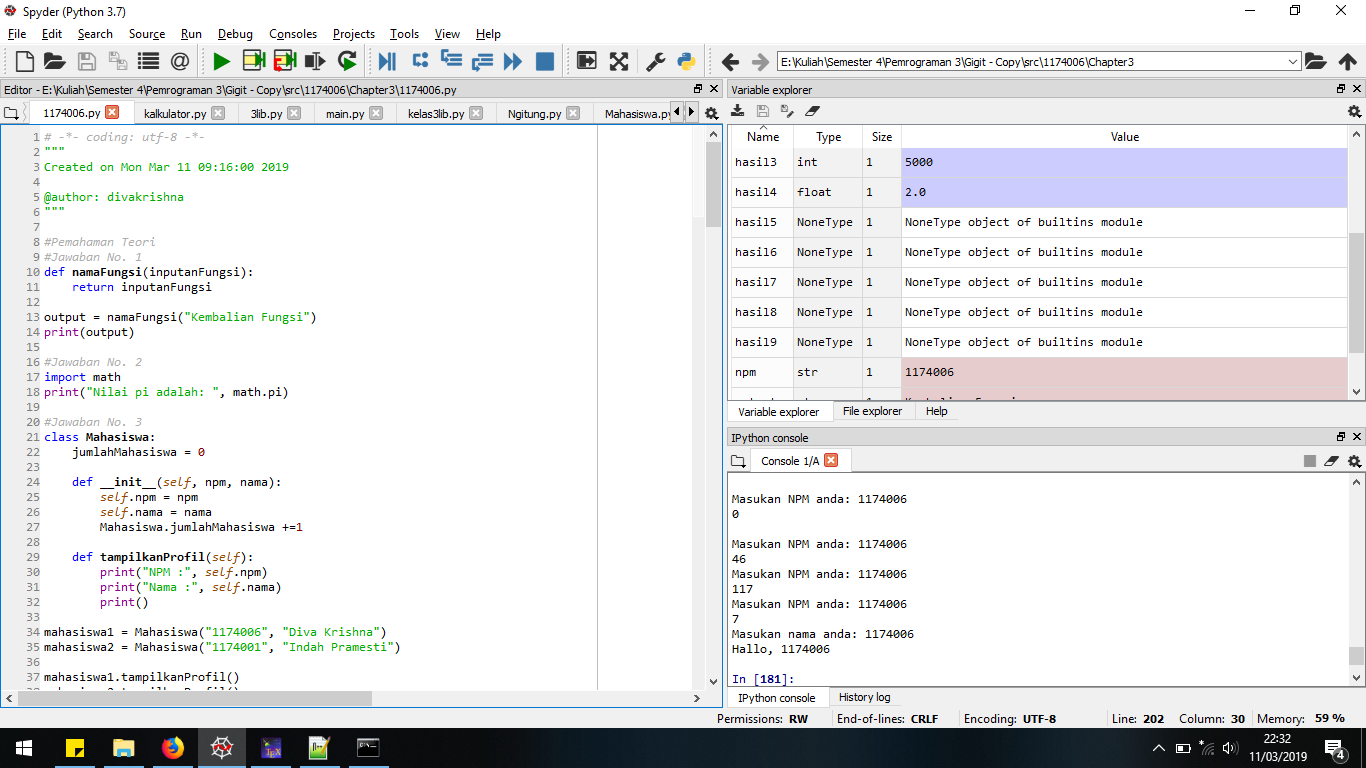
\includegraphics[width=10cm]{figures/diva/Chapter3/1174006_1.png}
	\centering
\end{figure}
\begin{figure}[H]
	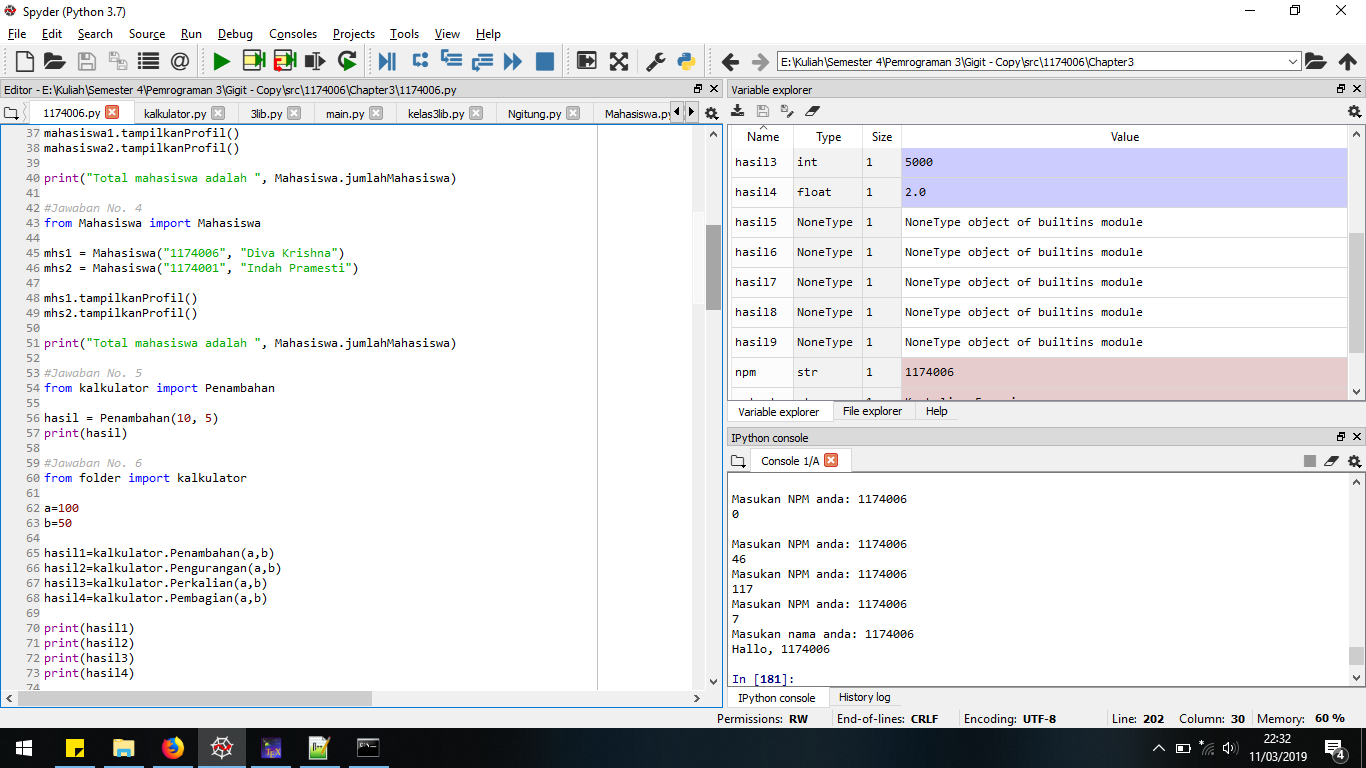
\includegraphics[width=10cm]{figures/diva/Chapter3/1174006_2.png}
	\centering
\end{figure}
\begin{figure}[H]
	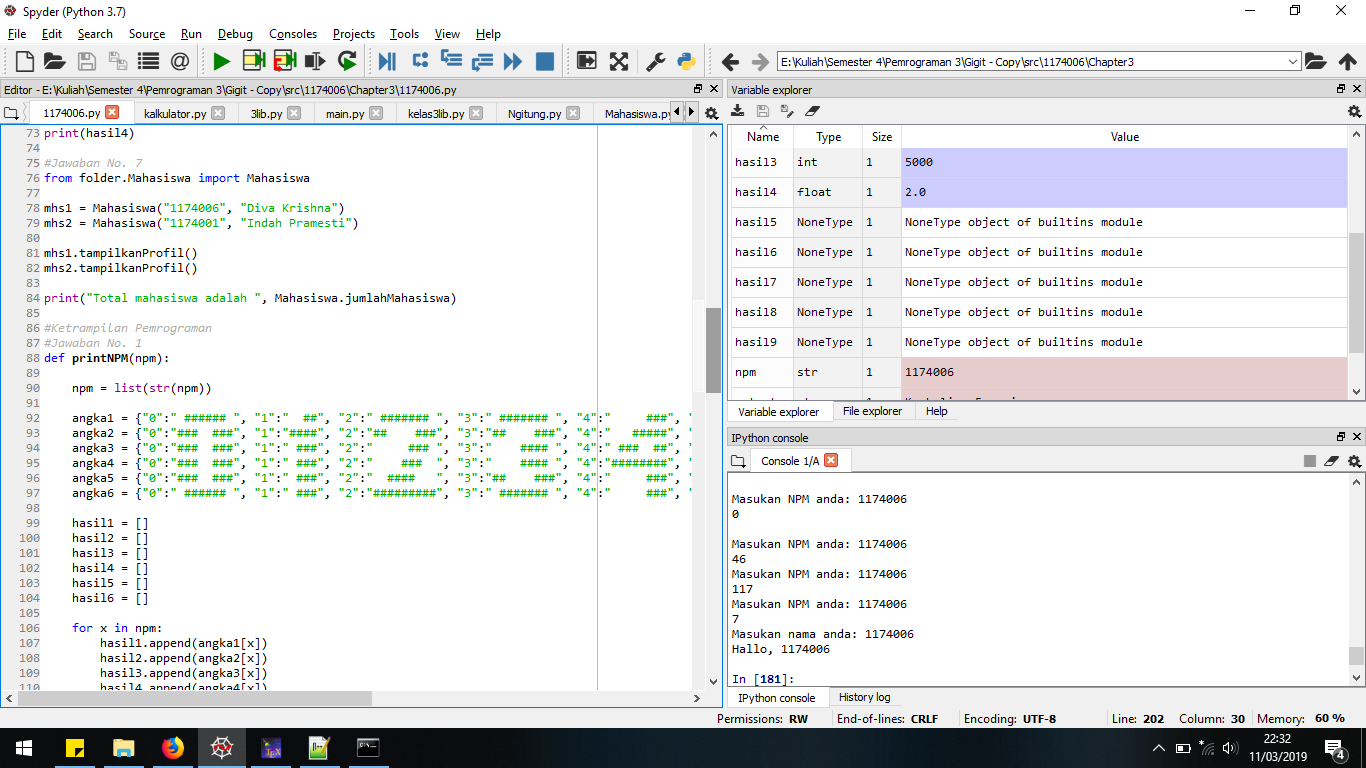
\includegraphics[width=10cm]{figures/diva/Chapter3/1174006_3.png}
	\centering
\end{figure}
\begin{figure}[H]
	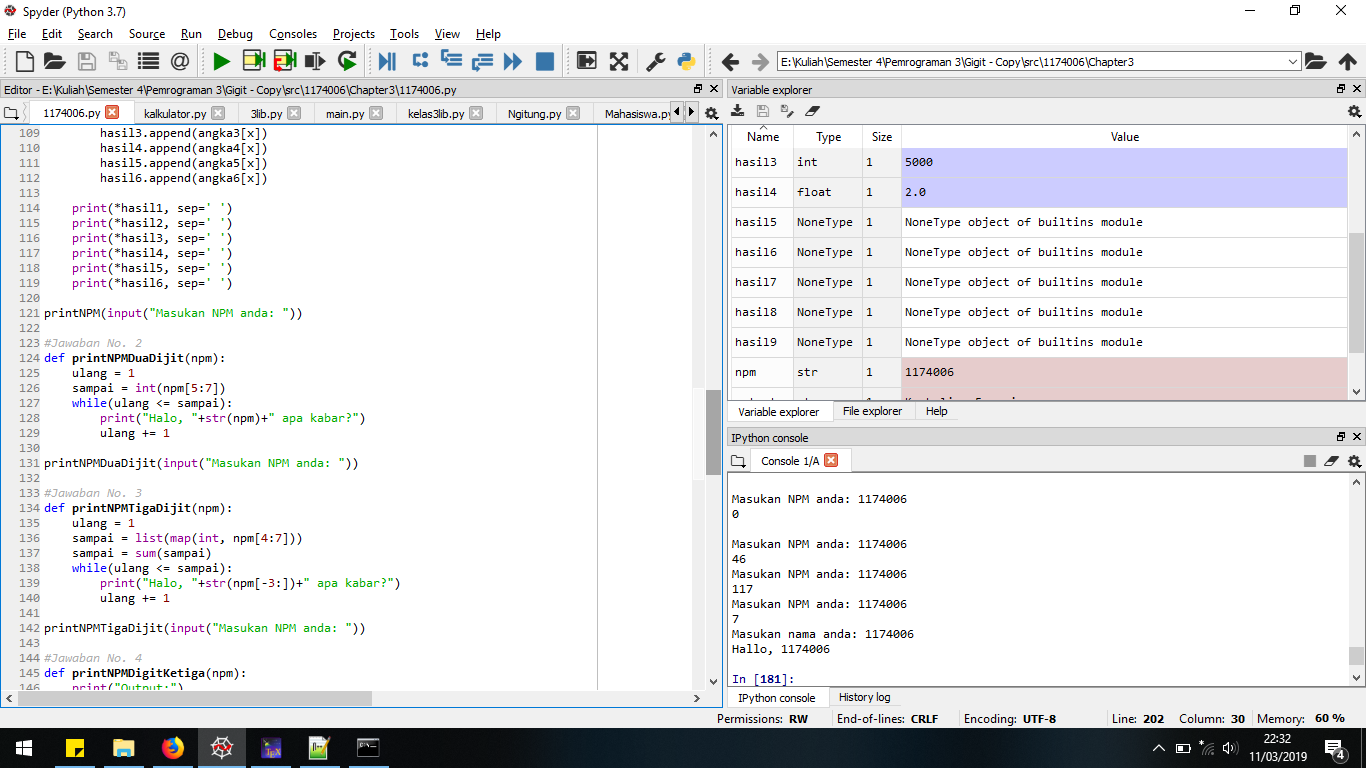
\includegraphics[width=10cm]{figures/diva/Chapter3/1174006_4.png}
	\centering
\end{figure}
\begin{figure}[H]
	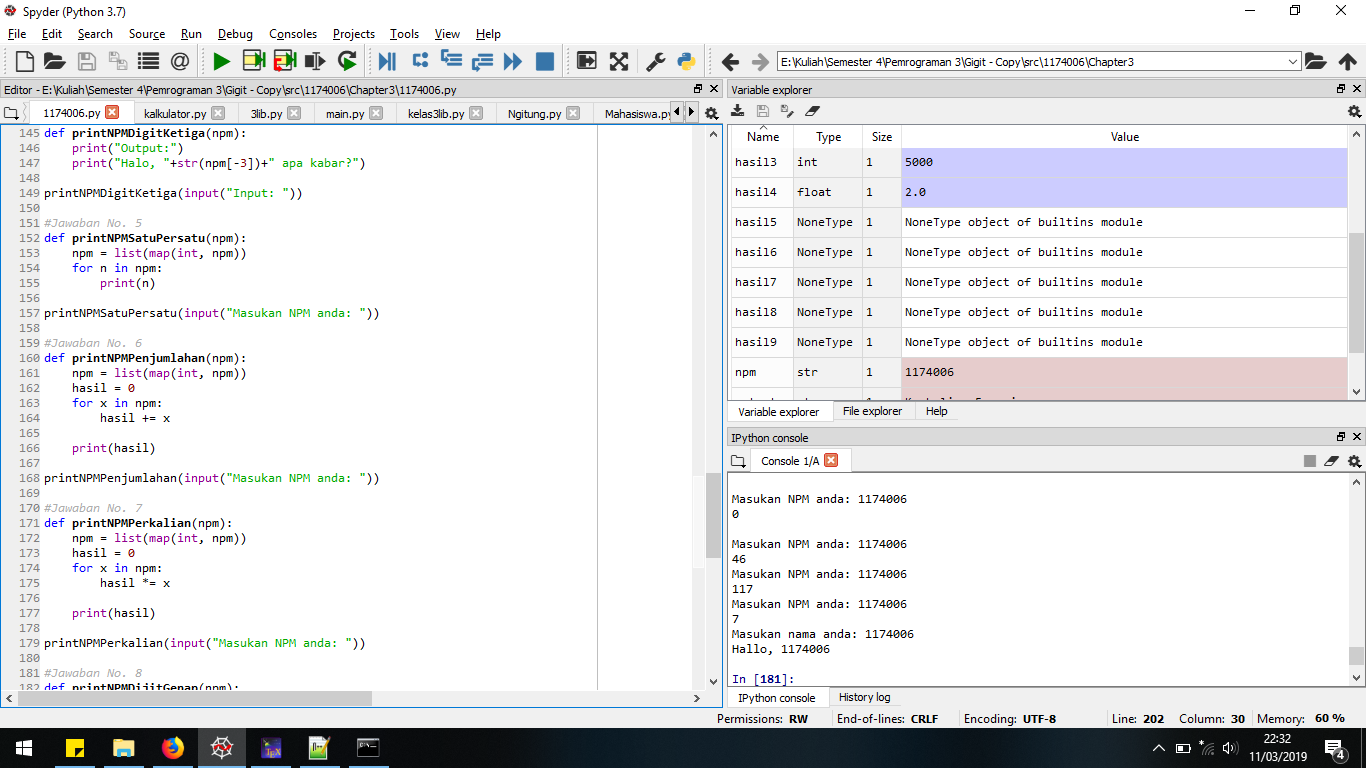
\includegraphics[width=10cm]{figures/diva/Chapter3/1174006_5.png}
	\centering
\end{figure}
\begin{figure}[H]
	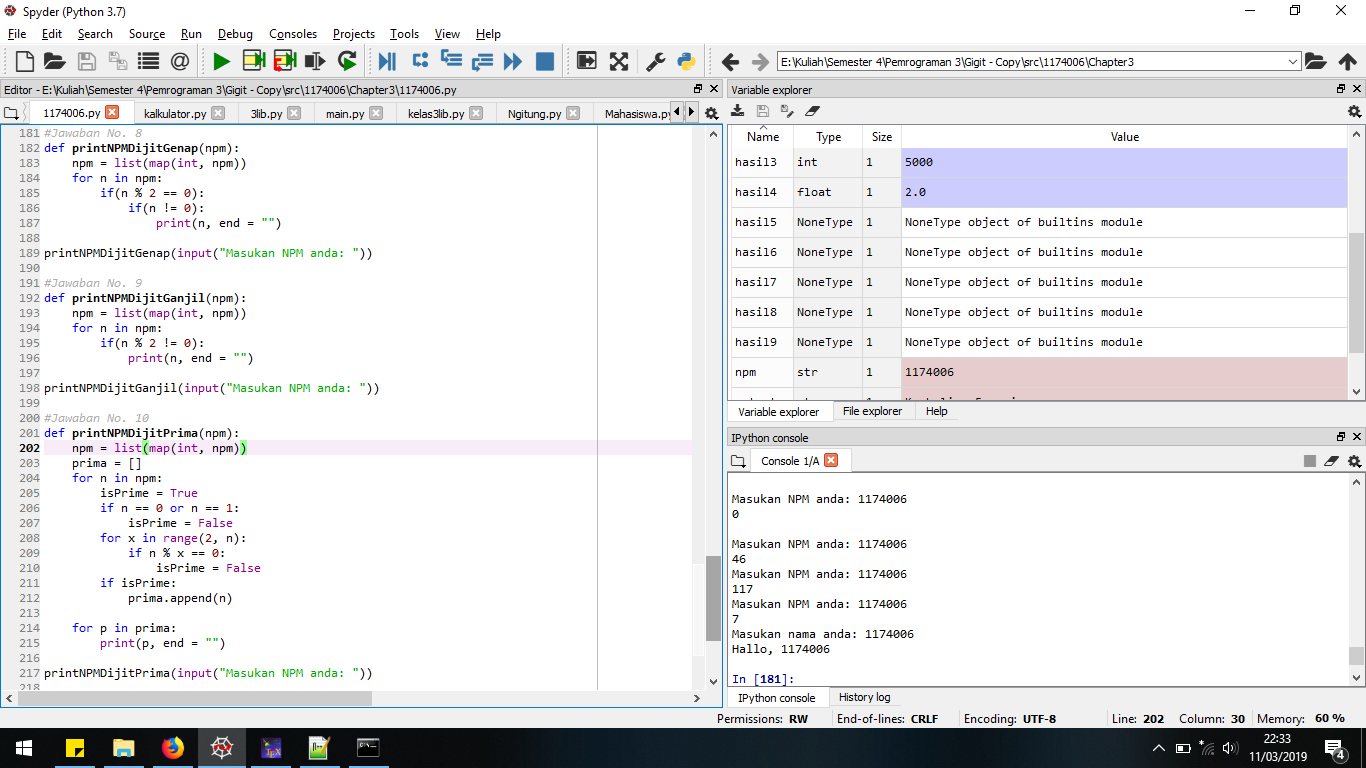
\includegraphics[width=10cm]{figures/diva/Chapter3/1174006_6.png}
	\centering
\end{figure}
\begin{figure}[H]
	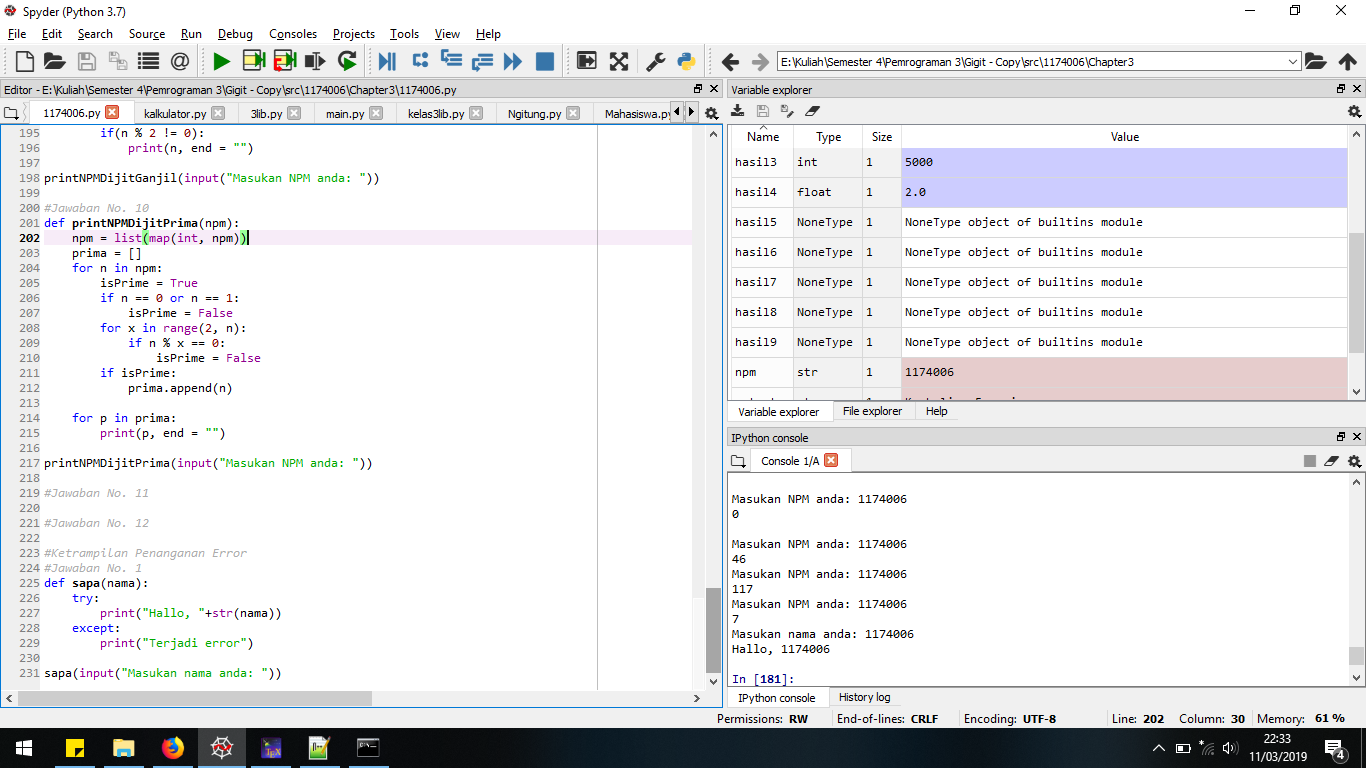
\includegraphics[width=10cm]{figures/diva/Chapter3/1174006_7.png}
	\centering
\end{figure}

\item Screenshoot Kodingan 3lib.py
\begin{figure}[H]
	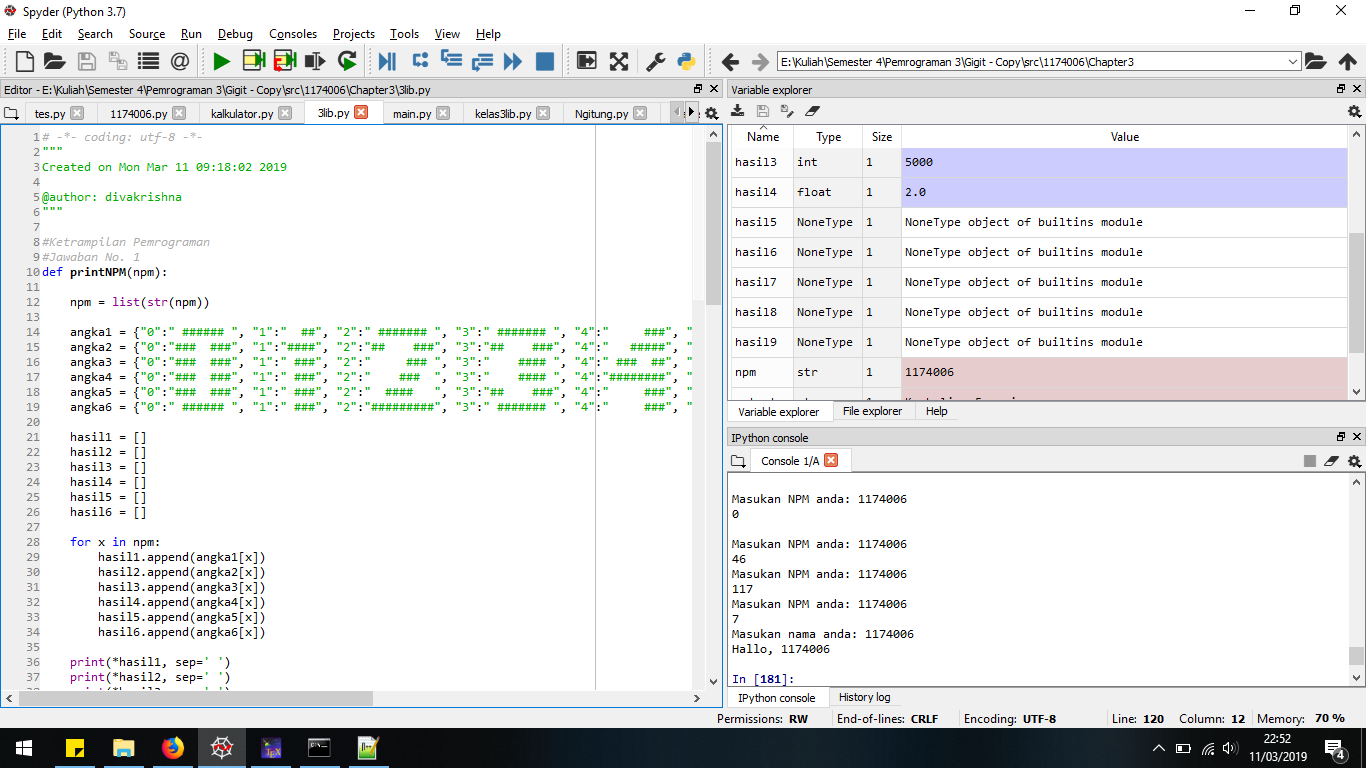
\includegraphics[width=10cm]{figures/diva/Chapter3/3lib_1.png}
	\centering
\end{figure}
\begin{figure}[H]
	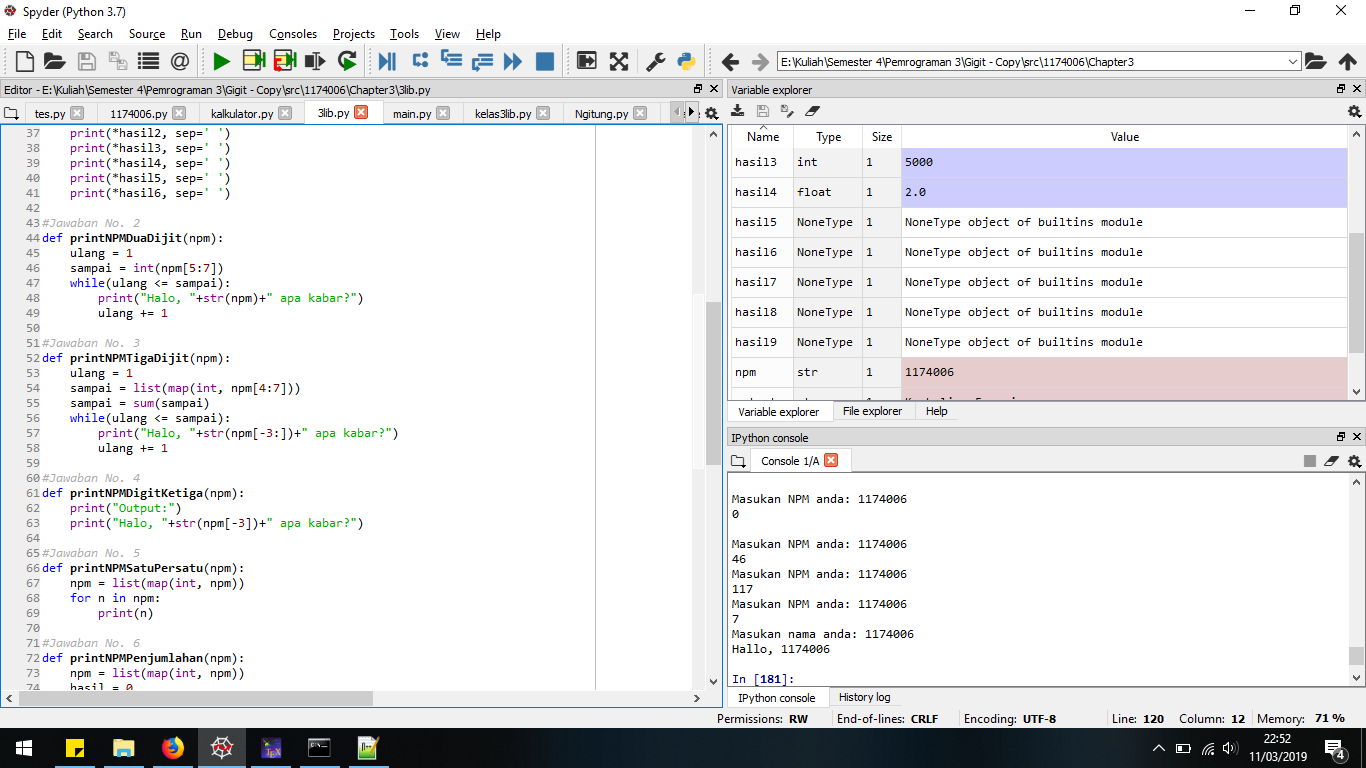
\includegraphics[width=10cm]{figures/diva/Chapter3/3lib_2.png}
	\centering
\end{figure}
\begin{figure}[H]
	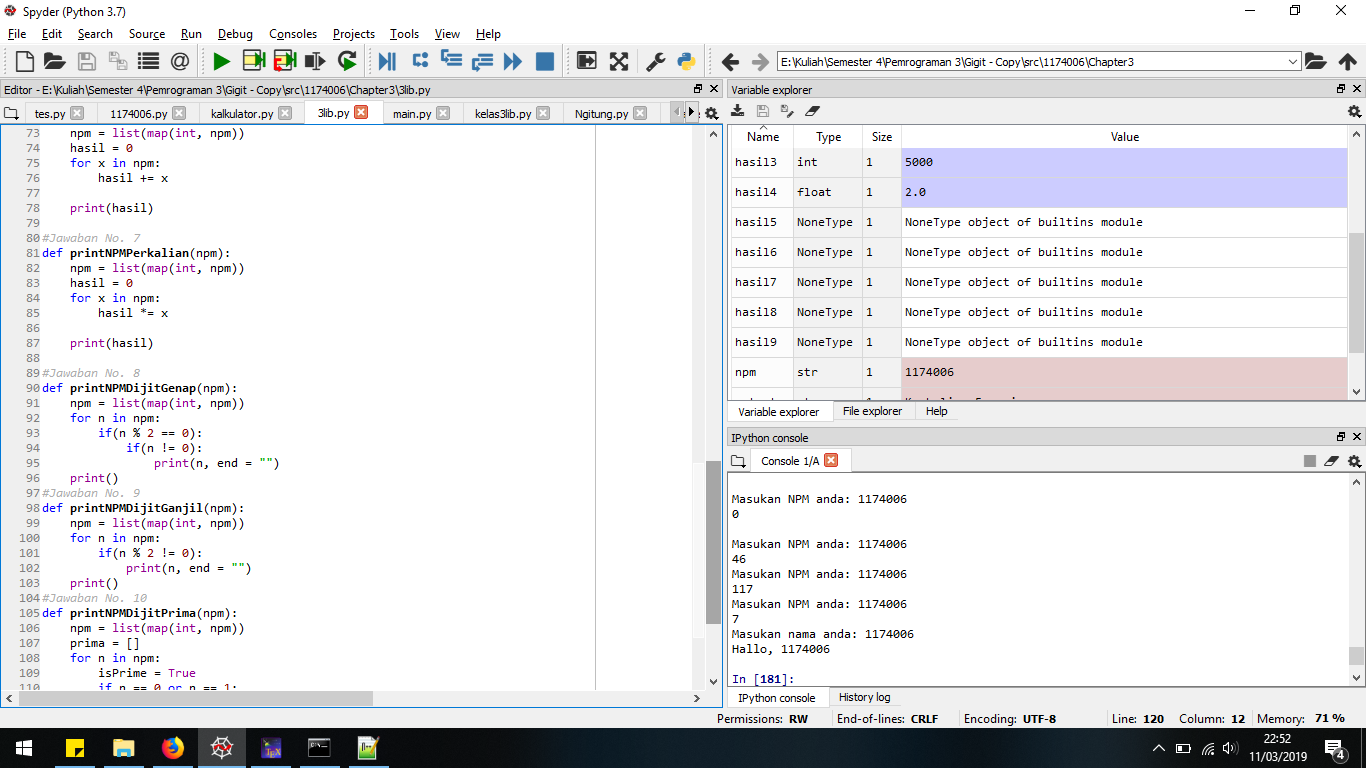
\includegraphics[width=10cm]{figures/diva/Chapter3/3lib_3.png}
	\centering
\end{figure}
\begin{figure}[H]
	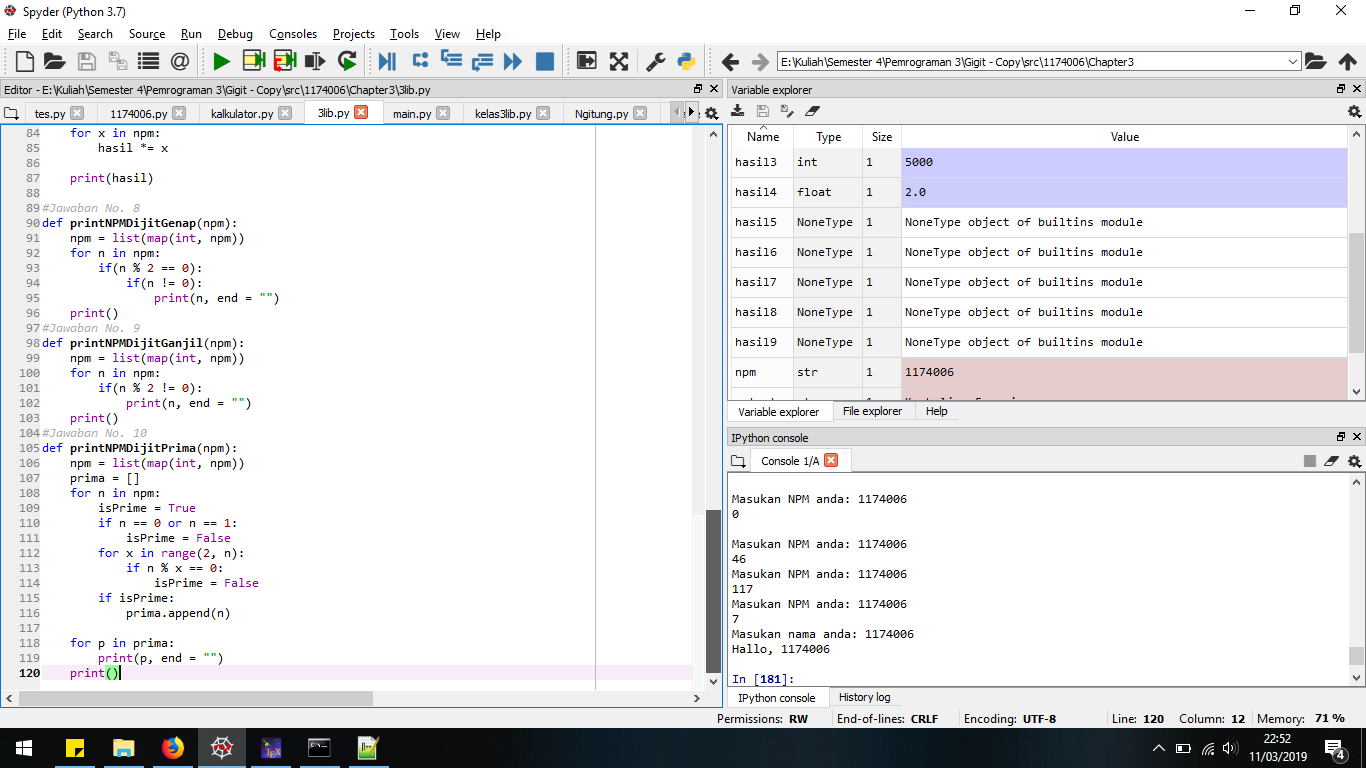
\includegraphics[width=10cm]{figures/diva/Chapter3/3lib_4.png}
	\centering
\end{figure}

\item Screenshoot Kodingan kelas3lib.py
\begin{figure}[H]
	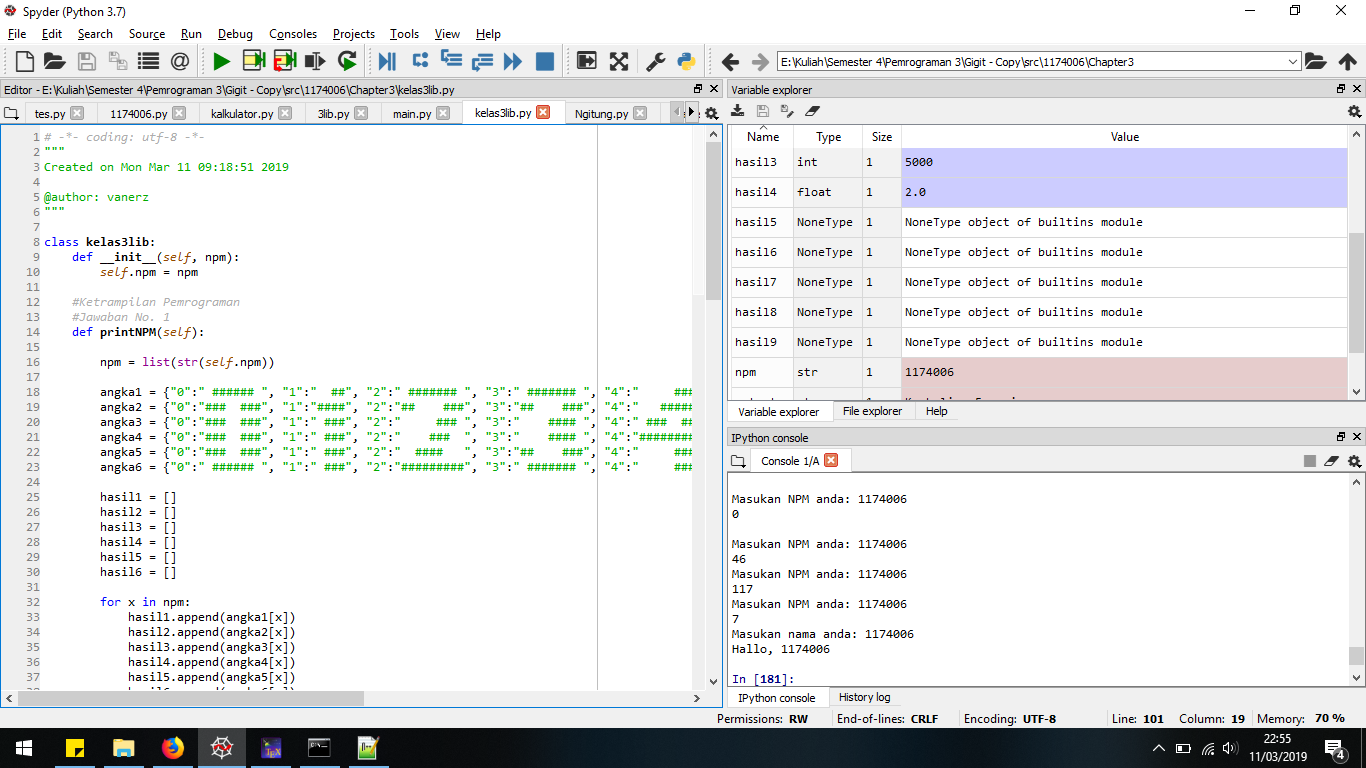
\includegraphics[width=10cm]{figures/diva/Chapter3/kelas3lib_1.png}
	\centering
\end{figure}
\begin{figure}[H]
	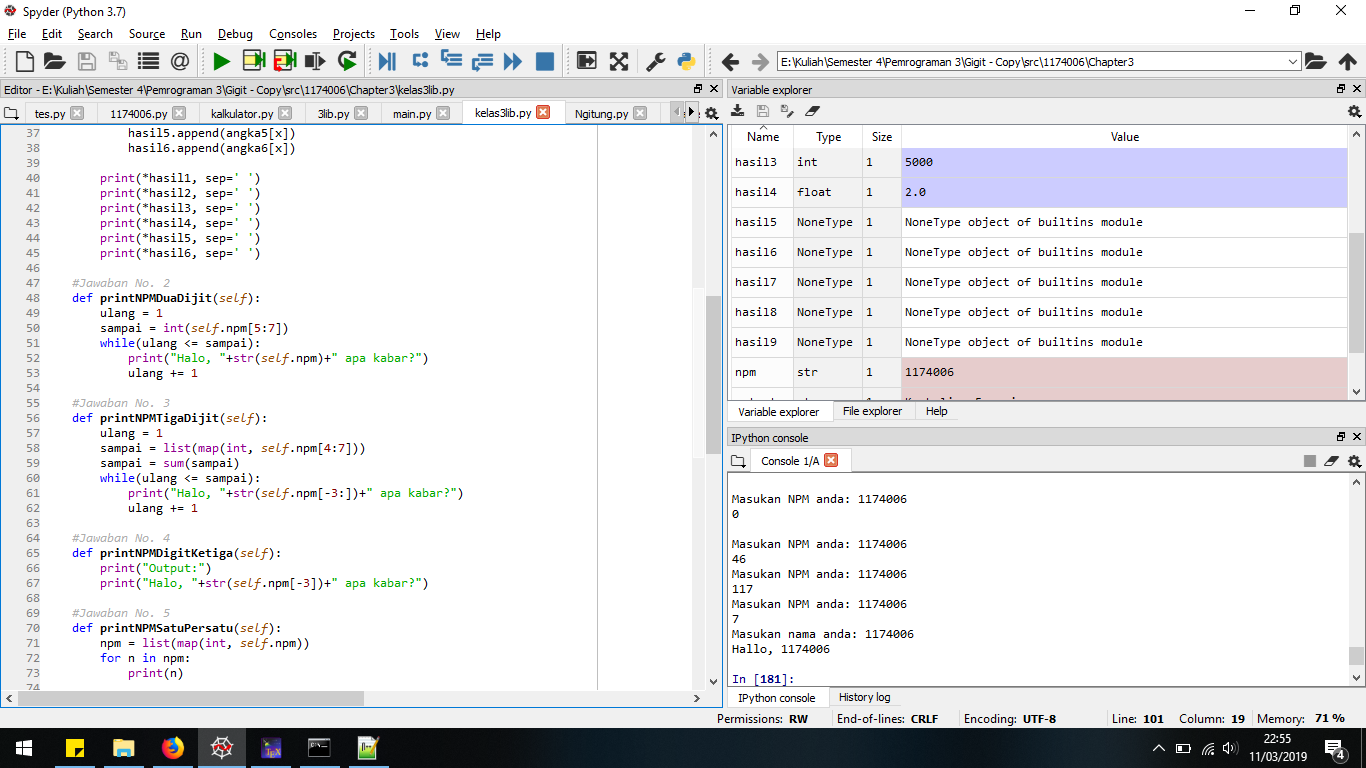
\includegraphics[width=10cm]{figures/diva/Chapter3/kelas3lib_2.png}
	\centering
\end{figure}
\begin{figure}[H]
	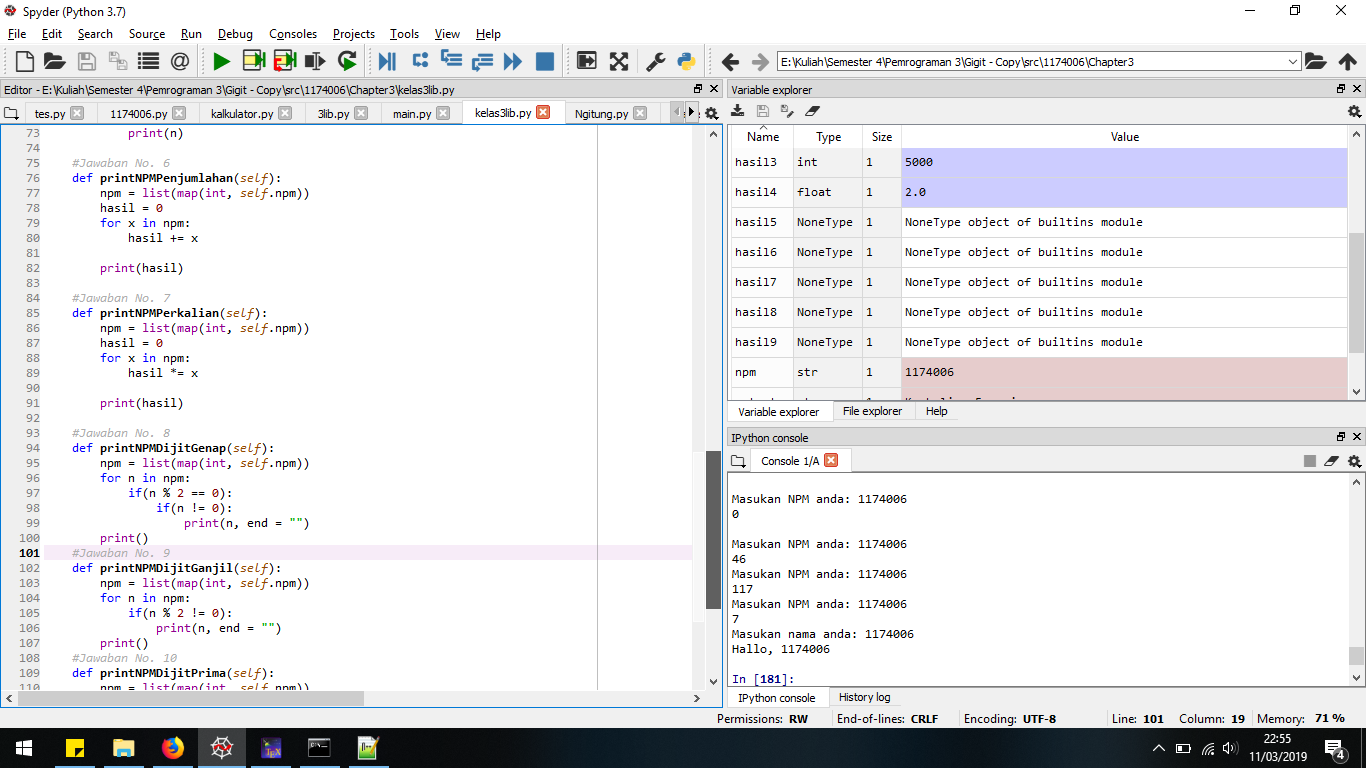
\includegraphics[width=10cm]{figures/diva/Chapter3/kelas3lib_3.png}
	\centering
\end{figure}
\begin{figure}[H]
	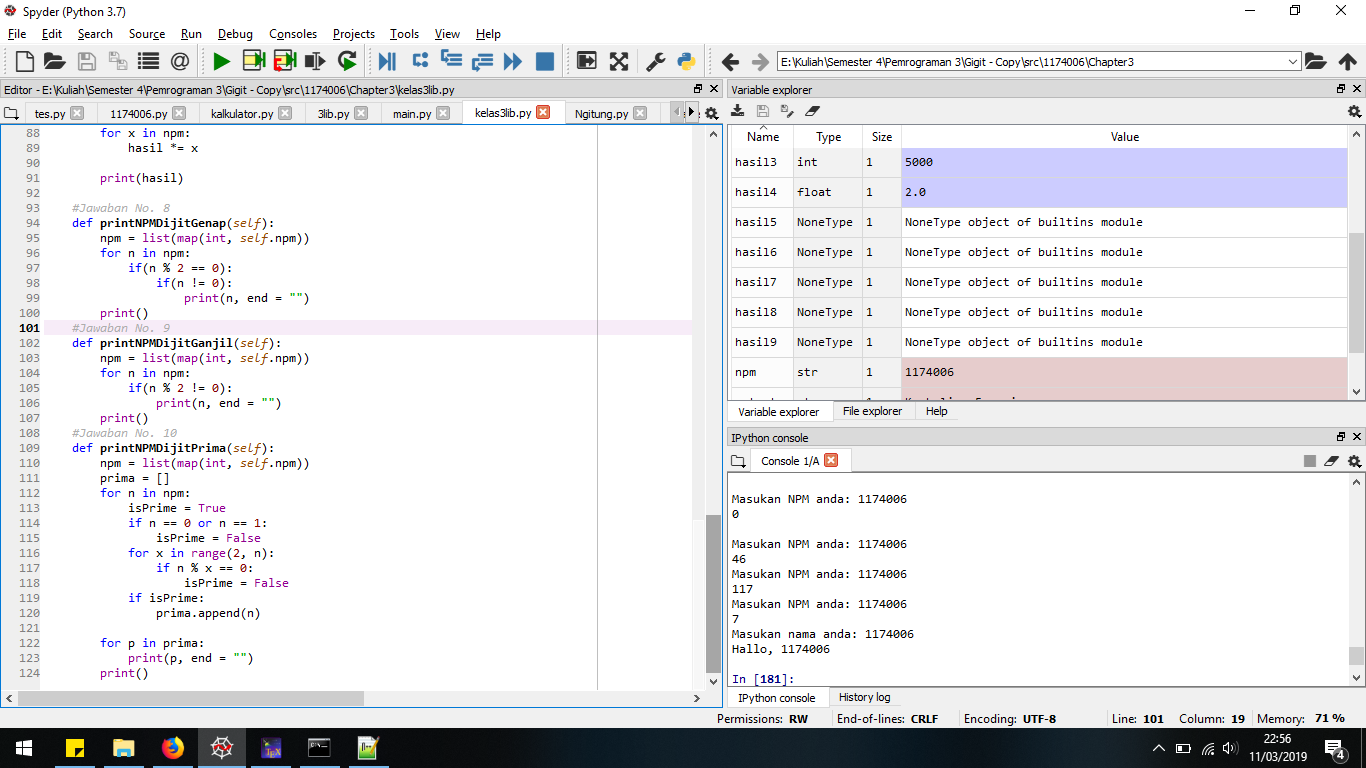
\includegraphics[width=10cm]{figures/diva/Chapter3/kelas3lib_4.png}
	\centering
\end{figure}

\item Screenshoot Kodingan main.py
\begin{figure}[H]
	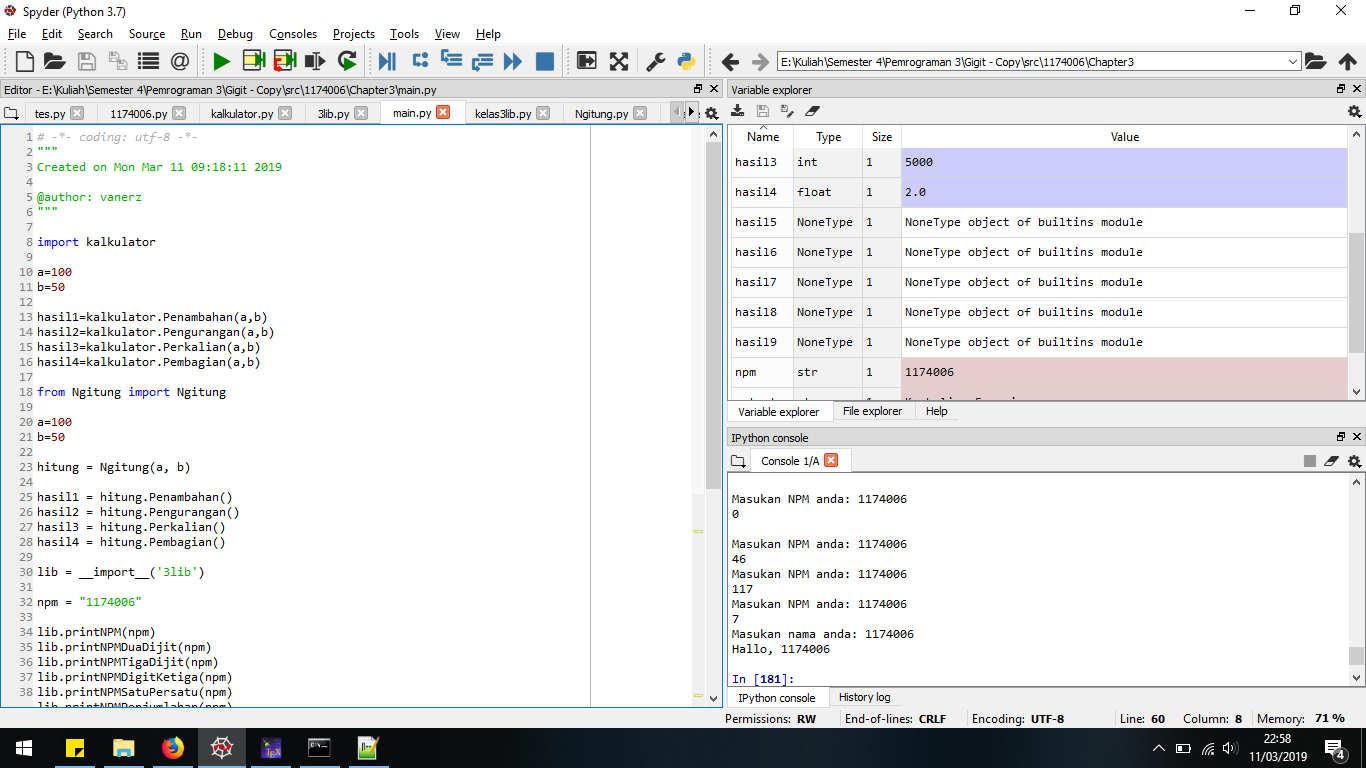
\includegraphics[width=10cm]{figures/diva/Chapter3/main_1.png}
	\centering
\end{figure}
\begin{figure}[H]
	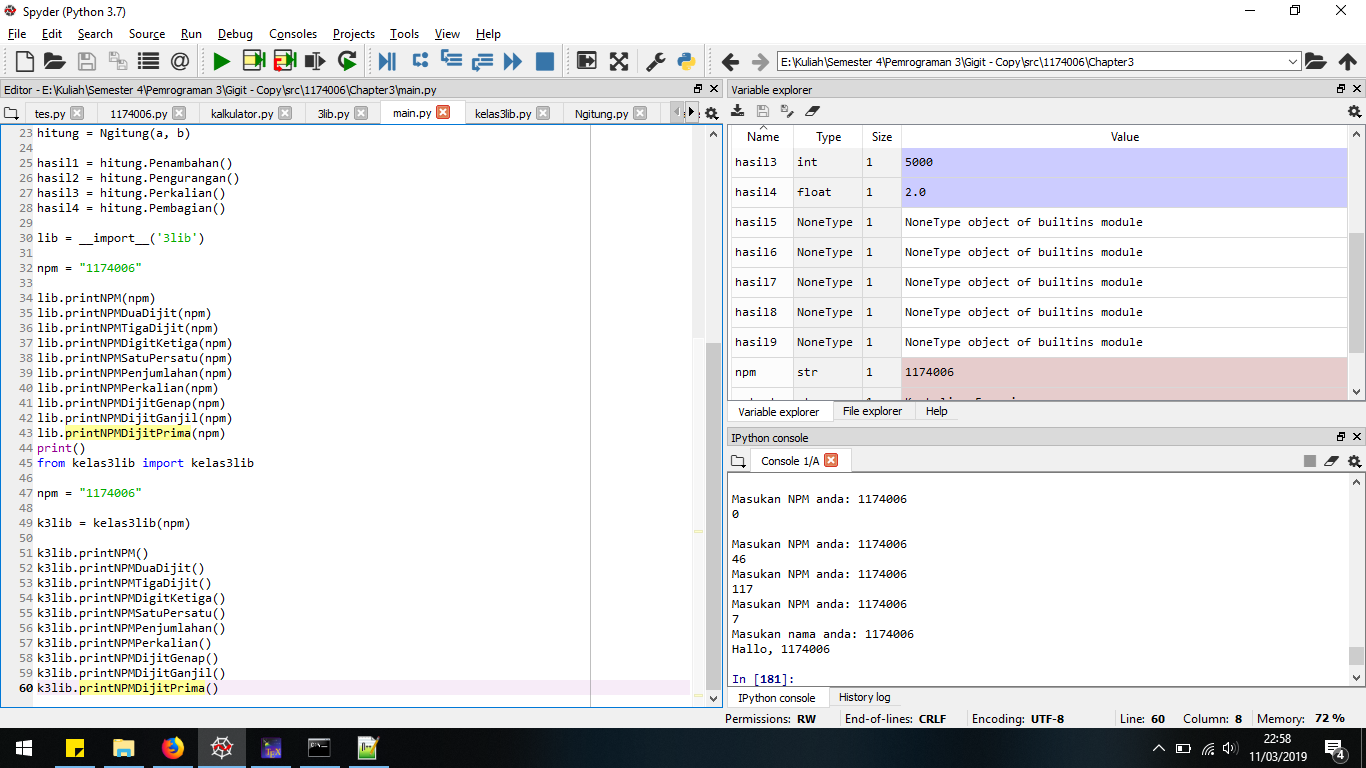
\includegraphics[width=10cm]{figures/diva/Chapter3/main_2.png}
	\centering
\end{figure}

\item Screenshoot Plagiarisme
\begin{figure}[H]
	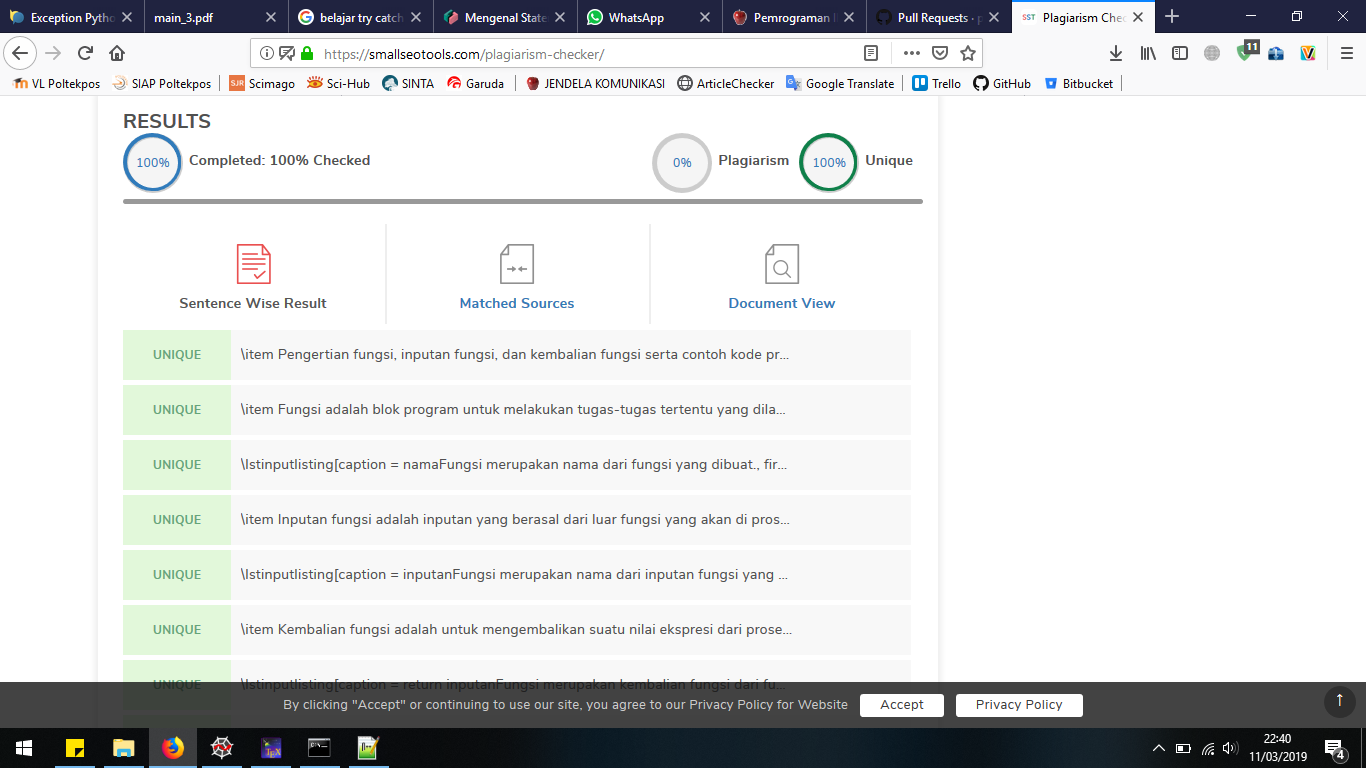
\includegraphics[width=10cm]{figures/diva/Chapter3/plagiarisme.png}
	\centering
\end{figure}
\end{enumerate}
%%%%%%%%%%%%%%%%%%%%%%%%%%%%%%%%%%%%%%%%%%%%%%%%%%%%%%%%%%%%%%
\section{Felix Setiawan Lase}
\subsubsection{Pemahanan Teori}
\begin{enumerate}
    \item Apa itu fungsi, inputan fungsi dan kembalian fungsi dengan contoh kode program
    lainnya.
    Fungsi adalah bagian dari program yang dapat digunakan ulang.
    Berikut merupakan contoh fungsi dan cara pemanggilannya
    \lstinputlisting[firstline=124, lastline=127]{src/1174026.py}

    Fungsi dapat membaca parameter, parameter adalah nilai yang disediakan kepada fungsi, dimana nilai ini akan menentukan output yang akan dihasilkan fungsi.
    \lstinputlisting[firstline=129, lastline=132]{src/1174026.py}

    Statemen return digunakan untuk keluar dari fungsi. Kita juga dapat menspesifikasikan nilai kembalian.
    \lstinputlisting[firstline=134, lastline=141]{src/1174026.py}

    \item Apa itu paket dan cara pemanggilan paket atau library dengan contoh kode
    program lainnya.
    Untuk memudahkan dalam pemanggilan fungsi yang di butuhkan, agar dapat dipanggil berulang.
    Cara pemanggilannya
    \lstinputlisting[firstline=143, lastline=144]{src/1174026.py}

    \item Jelaskan Apa itu kelas, apa itu objek, apa itu atribut, apa itu method dan
    contoh kode program lainnya masing-masing.
    kelas merupakan sebuah blueprint yang mepresentasikan objek.
    objek adalah hasil cetakan dadri sebuah kelas.
    method adalah suatu upaya yang digunakan oleh object.
    \lstinputlisting[firstline=146, lastline=168]{src/1174026.py}

    \item Jelaskan cara pemanggikan library kelas dari instansiasi dan pemakaiannya den-
    gan contoh program lainnya.
    Cara Pemanggilanya 
    \begin{itemize}
        \item pertama import terlebih dahulu filenya.
        \item kemudian buat variabel untuk menampung datanya
        \item setelah itu panggil nama classnya dan panggil methodnya
        \item Gunakan perintah print untuk menampilkan hasilnya

    \end{itemize}
    \lstinputlisting[firstline=170, lastline=175]{src/1174026.py}

    \item Jelaskan dengan contoh pemakaian paket dengan perintah from kalkulator im-
    port Penambahan disertai dengan contoh kode lainnya.
    Penggunaan paket from namafile import, itu berfungsi untuk memanggil file dan fungsinya
    \lstinputlisting[firstline=143, lastline=144]{src/1174026.py}

    \item Jelaskan dengan contoh kodenya, pemakaian paket fungsi apabila le library
    ada di dalam folder.
    Pemakaian paket adalah perkumpulan fungsi-fungsi. contoh kodenya adalah sebagai berikut :

    \item Jelaskan dengan contoh kodenya, pemakaian paket kelas apabila le library ada
    di dalam folder.
    \lstinputlisting[firstline=184, lastline=184]{src/1174026.py}

\end{enumerate}
\subsubsection{Ketrampilan Pemrograman}
\begin{enumerate}
    \item Buatlah fungsi dengan inputan variabel NPM, dan melakukan print luaran huruf
    yang dirangkai dari tanda bintang, pagar atau plus dari NPM kita. Tanda
    bintang untuk NPM mod 3=0, tanda pagar untuk NPM mod 3 =1, tanda plus
    untuk NPM mod3=2.
    \lstinputlisting[firstline=184, lastline=234]{src/1174026.py}

    \item Buatlah fungsi dengan inputan variabel berupa NPM. kemudian dengan meng-
    gunakan perulangan mengeluarkan print output sebanyak dua dijit belakang
    NPM.
    \lstinputlisting[firstline=237, lastline=243]{src/1174026.py}

    \item Buatlah fungsi dengan dengan input variabel string bernama NPM dan beri
    luaran output dengan perulangan berupa tiga karakter belakang dari NPM se-
    banyak penjumlahan tiga dijit tersebut.
    \lstinputlisting[firstline=245, lastline=255]{src/1174026.py}

    \item Buatlah fungsi hello word dengan input variabel string bernama NPM dan
    beri luaran output berupa digit ketiga dari belakang dari variabel NPM meng-
    gunakan akses langsung manipulasi string pada baris ketiga dari variabel NPM.
    \lstinputlisting[firstline=257, lastline=263]{src/1174026.py}

    \item buat fungsi program dengan input variabel NPM dan melakukan print nomor npm satu persatu kebawah.
    \lstinputlisting[firstline=265, lastline=269]{src/1174026.py}

    \item Buatlah fungsi dengan inputan variabel NPM, didalamnya melakukan penjum-
    lahan dari seluruh dijit NPM tersebut, wajib menggunakan perulangan dan
    atau kondisi.
    \lstinputlisting[firstline=272, lastline=279]{src/1174026.py}

    \item Buatlah fungsi dengan inputan variabel NPM, didalamnya melakukan melakukan
    perkalian dari seluruh dijit NPM tersebut, wajib menggunakan perulangan dan
    atau kondisi.
    \lstinputlisting[firstline=281, lastline=288]{src/1174026.py}

    \item Buatlah fungsi dengan inputan variabel NPM, Lakukan print NPM anda tapi
    hanya dijit genap saja. wajib menggunakan perulangan dan atau kondisi.
    \lstinputlisting[firstline=290, lastline=296]{src/1174026.py}

    \item Buatlah fungsi dengan inputan variabel NPM, Lakukan print NPM anda tapi
    hanya dijit ganjil saja. wajib menggunakan perulangan dan atau kondisi.
    \lstinputlisting[firstline=298, lastline=304]{src/1174026.py}

    \item Buatlah fungsi dengan inputan variabel NPM, Lakukan print NPM anda tapi
    hanya dijit yang termasuk bilangan prima saja. wajib menggunakan perulangan
    dan atau kondisi.
    \lstinputlisting[firstline=306, lastline=320]{src/1174026.py}

    \item Buatlah satu library yang berisi fungsi-fungsi dari nomor diatas dengan nama
    le 3lib.py dan berikan contoh cara pemanggilannya pada le main.py.
    \lstinputlisting[firstline=7, lastline=7]{src/main.py}

    \item Buatlah satu library class dengan nama le kelas3lib.py yang merupakan mod-
    ikasi dari fungsi-fungsi nomor diatas dan berikan contoh cara pemanggilannya
    pada le main.py.
    \lstinputlisting[firstline=8, lastline=9]{src/main.py}
    
\end{enumerate}
\subsubsection{Ketrampilan Penanganan Error}
Error yang di dapat dari mengerjakan tugas ini adalah type error, cara menaggulaginya dengan cara mengecheck kembali codingannya
kemudian run kembali aplikasinya
berikut contoh Penggunaan fungsi try dan exception
\lstinputlisting[firstline=177, lastline=182]{src/1174026.py}


%%%%%%%%%%%%%%%%%%%%%%%%%%%%%%%%%


\section{Dwi Septiani Tsaniyah}
\begin{enumerate}
    \item Apa itu fungsi, inputan fungsi dan kembalian fungsi dengan contoh kode program lainnya.
Fungsi memiliki tujuan agar kita dapat memecah program besar menjadi sub-sub program yang lebih sederhana. Pada saat kita membutuhkan suatu fitur maka kita tinggal memanggil fungsi yang telah kita buat. Fungsi pada python dibuat dengan kata kunci def dan diikuti dengan nama fungsi yang kita buat seperti contoh dibawah :
 \lstinputlisting[firstline=9, lastline=9]{src/1174003/1174003.py}

Inputan fungsi merupakan masukan yang kita berikan pada program dan program akan menampilkan hasil dari inputan yang kita masukkan. contoh dari inputan fungsi sebagai berikut :
 \lstinputlisting[firstline=12, lastline=14]{src/1174003/1174003.py}
Pengembalian fungsi memiliki tujuan untuk mengembalikan nilai dari hasil yang telah di proses. Dalam hal ini menggunakan kata kunci return yang diikuti dengan nilai atau variabel yang akan dikembalikan.
 \lstinputlisting[firstline=10, lastline=10]{src/1174003/1174003.py}

    \item Apa itu paket dan cara pemanggilan paket atau library dengan contoh kode program lainnya.
Library atau paket adalah modul-modul yang menyusun python. Modul-modul tersebut ditulis oleh berbagai orang dari seluruh dunia dan memiliki fungsi masing-masing untuk melakukan suatu hal. contoh kode programnya adalah sebagai berikut : from bte import penulisan print (penulisan(int(input(''Masukan NPM : ''))))
 \lstinputlisting[firstline=10, lastline=20]{src/1174003/1174003.py}

    \item Jelaskan Apa itu kelas, apa itu objek, apa itu atribut, apa itu method dan contoh kode program lainnya masing-masing.
kelas adalah Prototype yang ditentukan oleh pengguna untuk objek yang mendefinisikan seperangkat atribut yang menjadi ciri objek kelas apa pun. Objek ialah instansiasi atau perwujudan dari sebuah kelas. Bila kelas adalah prototipenya, dan objek adalah barang jadinya. Attribute adalah menggambarkan data yang dapat memberikan informasi kelas atau objek dimana attribut tersebut berada.
 \lstinputlisting[firstline=19, lastline=29]{src/1174003/1174003.py}

    \item Jelaskan cara pemanggilan library kelas dari instansiasi dan pemakaiannya dengan contoh program lainnya.
cara pemanggilan  library kelas dari instansiasi dan pemakaiannya adalah dengan cara meng-import library yang ada di dalam satu folder dan menggunakan kode berikut :
 \lstinputlisting[firstline=30, lastline=40]{src/1174003/1174003.py}

    \item Jelaskan dengan contoh pemakaian paket dengan perintah from kalkulator import Penambahan disertai dengan contoh kode lainnya.
contoh kodenya adalah sebagai berikut :
 \lstinputlisting[firstline=60, lastline=85]{src/1174003/1174003.py}

    \item Jelaskan dengan contoh kodenya, pemakaian paket fungsi apabila file library ada di dalam folder.
 Pemakaian paket adalah perkumpulan fungsi-fungsi. contoh kodenya adalah sebagai berikut :
 \lstinputlisting[firstline=90, lastline=100]{src/1174003/1174003.py}

    \item Jelaskan dengan contoh kodenya, pemakaian paket kelas apabila file library ada di dalam folder.
 \lstinputlisting[firstline=133, lastline=142]{src/1174003/1174003.py}
 \end{enumerate}

%%%%%%%%%%%%%%%%%%%%%%%%%%%%%%%%%%%%%%%%%%%%%%%%

\section{Dwi Yulianingsih}
\subsection{Pemahaman Teori}
\begin{enumerate}
    \item Apa itu fungsi, inputan fungsi dan kembalian fungsi dengan contoh kode program lainnya.
Fungsi memiliki tujuan agar kita dapat memecah program besar menjadi sub-sub program yang lebih sederhana. Pada saat kita membutuhkan suatu fitur maka kita tinggal memanggil fungsi yang telah kita buat. Fungsi pada python dibuat dengan kata kunci def dan diikuti dengan nama fungsi yang kita buat seperti contoh dibawah :
 \lstinputlisting[firstline=9, lastline=9]{src/1174009/tugas.py}
Inputan fungsi merupakan masukan yang kita berikan pada program dan program akan menampilkan hasil dari inputan yang kita masukkan. contoh dari inputan fungsi sebagai berikut :
 \lstinputlisting[firstline=12, lastline=14]{src/1174009/tugas.py}
Pengembalian fungsi memiliki tujuan untuk mengembalikan nilai dari hasil yang telah di proses. Dalam hal ini menggunakan kata kunci return yang diikuti dengan nilai atau variabel yang akan dikembalikan.
 \lstinputlisting[firstline=10, lastline=10]{src/1174009/tugas.py}

    \item Apa itu paket dan cara pemanggilan paket atau library dengan contoh kode program lainnya.
Library atau paket adalah modul-modul yang menyusun python. Modul-modul tersebut ditulis oleh berbagai orang dari seluruh dunia dan memiliki fungsi masing-masing untuk melakukan suatu hal. contoh kode programnya adalah sebagai berikut :
 \lstinputlisting[firstline=16, lastline=20]{src/1174009/tugas.py}

    \item Jelaskan Apa itu kelas, apa itu objek, apa itu atribut, apa itu method dan contoh kode program lainnya masing-masing.
kelas adalah Prototype yang ditentukan oleh pengguna untuk objek yang mendefinisikan seperangkat atribut yang menjadi ciri objek kelas apa pun. Objek ialah instansiasi atau perwujudan dari sebuah kelas. Bila kelas adalah prototipenya, dan objek adalah barang jadinya. Atribut adalah data anggota (variabel kelas dan variabel contoh) dan metode, diakses melalui notasi titik. Sedangkan method fungsi yang didefinisikan di dalam suatu kelas.
 \lstinputlisting[firstline=23, lastline=32]{src/1174009/tugas.py}

    \item Jelaskan cara pemanggilan library kelas dari instansiasi dan pemakaiannya dengan contoh program lainnya.
cara pemanggilan  library kelas dari instansiasi dan pemakaiannya adalah dengan cara meng-import library yang ada di dalam satu folder dan menggunakan kode berikut :
 \lstinputlisting[firstline=34, lastline=40]{src/1174009/tugas.py}

    \item Jelaskan dengan contoh pemakaian paket dengan perintah from kalkulator import Penambahan disertai dengan contoh kode lainnya.
Penggunaan paket berfungsi untuk memanggil file dan fungsinya. contoh kodenya adalah sebagai berikut :
 \lstinputlisting[firstline=42, lastline=44]{src/1174009/tugas.py}

    \item Jelaskan dengan contoh kodenya, pemakaian paket fungsi apabila file library ada di dalam folder.
 Pemakaian paket adalah perkumpulan fungsi-fungsi. contoh kodenya adalah sebagai berikut :
 \lstinputlisting[firstline=46, lastline=55]{src/1174009/tugas.py}

    \item Jelaskan dengan contoh kodenya, pemakaian paket kelas apabila file library ada di dalam folder.
 \lstinputlisting[firstline=62, lastline=67]{src/1174009/tugas.py}

\end{enumerate}

\subsection{Praktek}
\begin{enumerate}
    \item jawaban no 1
 \lstinputlisting[firstline=8, lastline=43]{src/1174009/1174009.py}

    \item jawaban no 2
 \lstinputlisting[firstline=45, lastline=51]{src/1174009/1174009.py}

    \item jawaban no 3
 \lstinputlisting[firstline=53, lastline=61]{src/1174009/1174009.py}

    \item jawaban no 4
 \lstinputlisting[firstline=63, lastline=68]{src/1174009/1174009.py}

    \item jawaban no 5
 \lstinputlisting[firstline=70, lastline=75]{src/1174009/1174009.py}

    \item jawaban no 6
 \lstinputlisting[firstline=77, lastline=83]{src/1174009/1174009.py}

    \item jawaban no 7
 \lstinputlisting[firstline=85, lastline=91]{src/1174009/1174009.py}

    \item jawaban no 8
 \lstinputlisting[firstline=93, lastline=100]{src/1174009/1174009.py}

    \item jawaban no 9
 \lstinputlisting[firstline=103, lastline=108]{src/1174009/1174009.py}

    \item jawaban no 10
 \lstinputlisting[firstline=110, lastline=126]{src/1174009/1174009.py}

    \item jawaban 11
 \lstinputlisting[firstline=8, lastline=21]{src/1174009/main.py}

    \item jawaban 12
 \lstinputlisting[firstline=23, lastline=38]{src/1174009/main.py}
\end{enumerate}

\subsection{Penanganan Eror}
untuk menangani eror yang terjadi bisa menggunakan source kode dibawah ini :
 \lstinputlisting[firstline=69, lastline=75]{src/1174009/tugas.py}

\begin{figure}[!Htbp]
\centering
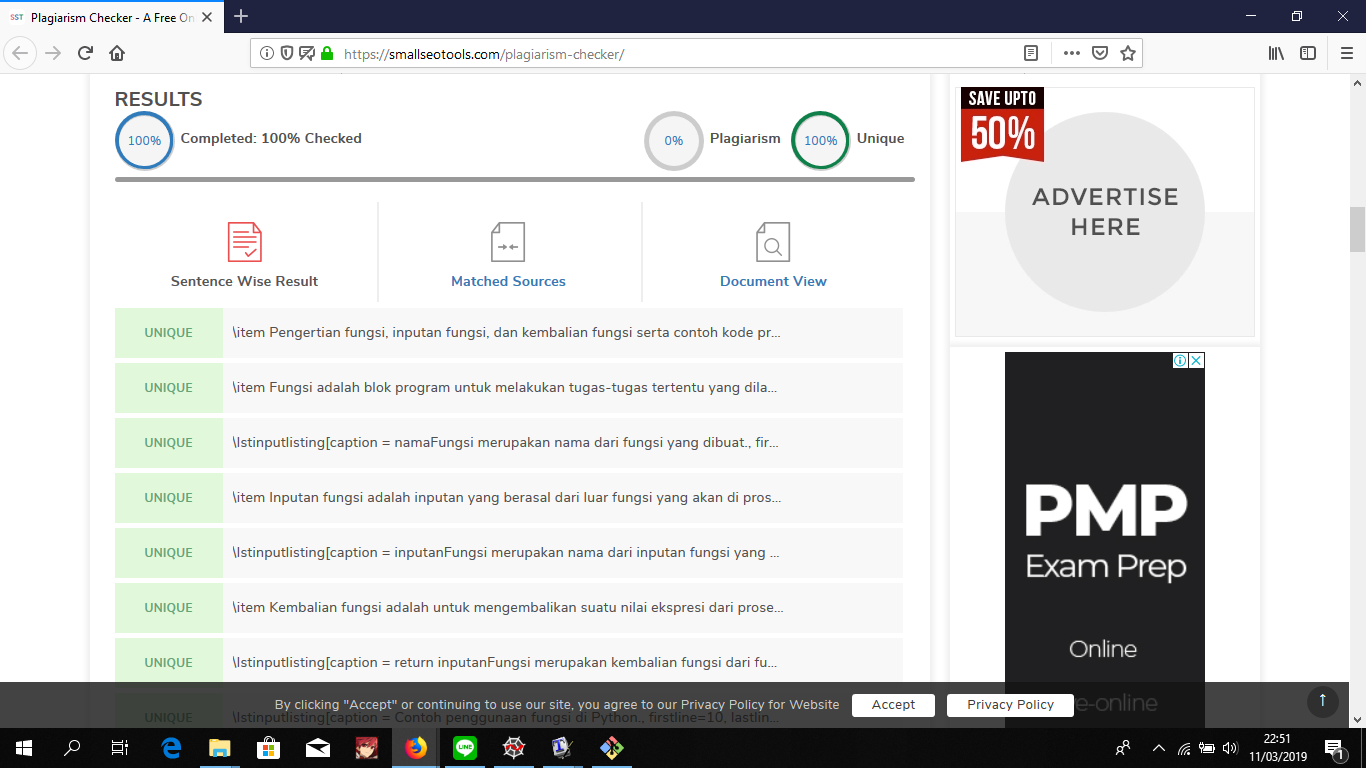
\includegraphics[width=6cm,height=6cm]{figures/Wiyul.png}
\caption{SS Bebas Plagiarisme}
\label{dwiyul}
\end{figure}
%%%%%%%%%%%%%%%%%%%%%%%%%%%%%%%%%%%%%%%%%%%%%%%%%%%%%%%%%%%%%%%%%%%%%%%%%%%%%%%%%%%%%%%%%%%%%%%%%%%%%%%%%%%%%%%%


\section{Choirul Anam}
\subsubsection{Pemahaman Teori}
\begin{enumerate}
    \item Apa itu fungsi, inputan fungsi dan kembalian fungsi dengan contoh kode program
    lainnya.
    Fungsi adalah suatu perintah diaman perintah tersebut dapat di panggil berulang ulang.
    Berikut merupakan contoh fungsi dan cara pemanggilannya
    \lstinputlisting[firstline=184, lastline=187]{src/1174004.py}

    Fungsi juga bisa membaca parameter, dimana parameter adalah nilai yang di inputkan atau di lemparkan untuk kebutuhan fungsi, dimana nilai ini akan menentukan output yang akan dihasilkan fungsi.
    \lstinputlisting[firstline=189, lastline=192]{src/1174004.py}

    Statemen return digunakan untuk keluar dari fungsi. Kita juga dapat menspesifikasikan nilai kembalian.
    \lstinputlisting[firstline=194, lastline=201]{src/1174004.py}

    \item Apa itu paket dan cara pemanggilan paket atau library dengan contoh kode
    program lainnya.
    Untuk memudahkan dalam pemanggilan fungsi yang di butuhkan, agar dapat dipanggil berulang.
    Cara pemanggilannya
    \lstinputlisting[firstline=203, lastline=204]{src/1174004.py}

    \item Jelaskan Apa itu kelas, apa itu objek, apa itu atribut, apa itu method dan
    contoh kode program lainnya masing-masing.
    kelas merupakan sebuah blueprint yang mepresentasikan objek.
    objek adalah hasil cetakan dadri sebuah kelas.
    method adalah suatu upaya yang digunakan oleh object.
    atribut adalah apasaja yang dapat dilakukan oleh objek
    \lstinputlisting[firstline=206, lastline=228]{src/1174004.py}

    \item Jelaskan cara pemanggilan library kelas dari instansiasi dan pemakaiannya den-
    gan contoh program lainnya.
    Cara Pemanggilanya 
    \begin{itemize}
        \item import file.
        \item kemudian buat variabel untuk menampung datanya
        \item setelah itu panggil nama classnya dan panggil methodnya
        \item Gunakan perintah print untuk menampilkan hasilnya

    \end{itemize}
    \lstinputlisting[firstline=230, lastline=235]{src/1174004.py}

    \item Jelaskan dengan contoh pemakaian paket dengan perintah from kalkulator im-
    port Penambahan disertai dengan contoh kode lainnya.
    Penggunaan paket from namafile import, itu berfungsi untuk memanggil file dan fungsinya
    \lstinputlisting[firstline=203, lastline=204]{src/1174004.py}

    \item Jelaskan dengan contoh kodenya, pemakaian paket fungsi apabila le library
    ada di dalam folder.
    Pemakaian paket adalah perkumpulan fungsi-fungsi. contoh kodenya adalah sebagai berikut :

    \item Jelaskan dengan contoh kodenya, pemakaian paket kelas apabila le library ada
    di dalam folder.
    \lstinputlisting[firstline=244, lastline=244]{src/1174004.py}

\end{enumerate}
\subsubsection{Ketrampilan Pemrograman}
\begin{enumerate}
    \item Buatlah fungsi dengan inputan variabel NPM, dan melakukan print luaran huruf
    yang dirangkai dari tanda bintang, pagar atau plus dari NPM kita. Tanda
    bintang untuk NPM mod 3=0, tanda pagar untuk NPM mod 3 =1, tanda plus
    untuk NPM mod3=2.
    \lstinputlisting[firstline=245, lastline=294]{src/1174004.py}

    \item Buatlah fungsi dengan inputan variabel berupa NPM. kemudian dengan meng-
    gunakan perulangan mengeluarkan print output sebanyak dua dijit belakang
    NPM.
    \lstinputlisting[firstline=297, lastline=303]{src/1174004.py}

    \item Buatlah fungsi dengan dengan input variabel string bernama NPM dan beri
    luaran output dengan perulangan berupa tiga karakter belakang dari NPM se-
    banyak penjumlahan tiga dijit tersebut.
    \lstinputlisting[firstline=306, lastline=315]{src/1174004.py}

    \item Buatlah fungsi hello word dengan input variabel string bernama NPM dan
    beri luaran output berupa digit ketiga dari belakang dari variabel NPM meng-
    gunakan akses langsung manipulasi string pada baris ketiga dari variabel NPM.
    \lstinputlisting[firstline=318, lastline=323]{src/1174004.py}

    \item buat fungsi program dengan input variabel NPM dan melakukan print nomor npm satu persatu kebawah.
    \lstinputlisting[firstline=326, lastline=330]{src/1174004.py}

    \item Buatlah fungsi dengan inputan variabel NPM, didalamnya melakukan penjum-
    lahan dari seluruh dijit NPM tersebut, wajib menggunakan perulangan dan
    atau kondisi.
    \lstinputlisting[firstline=333, lastline=339]{src/1174004.py}

    \item Buatlah fungsi dengan inputan variabel NPM, didalamnya melakukan melakukan
    perkalian dari seluruh dijit NPM tersebut, wajib menggunakan perulangan dan
    atau kondisi.
    \lstinputlisting[firstline=342, lastline=348]{src/1174004.py}

    \item Buatlah fungsi dengan inputan variabel NPM, Lakukan print NPM anda tapi
    hanya dijit genap saja. wajib menggunakan perulangan dan atau kondisi.
    \lstinputlisting[firstline=351, lastline=356]{src/1174004.py}

    \item Buatlah fungsi dengan inputan variabel NPM, Lakukan print NPM anda tapi
    hanya dijit ganjil saja. wajib menggunakan perulangan dan atau kondisi.
    \lstinputlisting[firstline=359, lastline=364]{src/1174004.py}

    \item Buatlah fungsi dengan inputan variabel NPM, Lakukan print NPM anda tapi
    hanya dijit yang termasuk bilangan prima saja. wajib menggunakan perulangan
    dan atau kondisi.
    \lstinputlisting[firstline=367, lastline=380]{src/1174004.py}

    \item Buatlah satu library yang berisi fungsi-fungsi dari nomor diatas dengan nama
    le 3lib.py dan berikan contoh cara pemanggilannya pada le main.py.
    \lstinputlisting[firstline=7, lastline=7]{src/main.py}

    \item Buatlah satu library class dengan nama le kelas3lib.py yang merupakan mod-
    ikasi dari fungsi-fungsi nomor diatas dan berikan contoh cara pemanggilannya
    pada le main.py.
    \lstinputlisting[firstline=8, lastline=9]{src/main.py}
    
\end{enumerate}
\subsubsection{Ketrampilan Penanganan Error}
Error yang di dapat dari mengerjakan tugas ini adalah type error, cara menaggulaginya dengan cara mengecheck kembali codingannya
kemudian run kembali aplikasinya
berikut contoh Penggunaan fungsi try dan exception
\lstinputlisting[firstline=177, lastline=182]{src/1174004.py}

%%%%%%%%%%%%%%%%%%%%%%%%%%%%%%%%%%%%%%%%%%%%%%%%%%%%%%%%%%%%%%
\section{Muh. Rifky Prananda}
\subsubsection{Pemahanan Teori}
\begin{enumerate}
    \item Apa itu fungsi, inputan fungsi dan kembalian fungsi dengan contoh kode program
    lainnya.
    Fungsi adalah salah satu bagian dari program yang dapat digunakan ulang.
    Berikut merupakan contoh fungsi dan cara pemanggilannya
    \lstinputlisting[firstline=74, lastline=77]{src/1174017.py}

    Fungsi bisa membaca parameter, parameter yaitu sebuah nilai yang tersedia untuk fungsi, dimana pada nilai ini menentukan output yang dihasilkan fungsi.
    \lstinputlisting[firstline=79, lastline=82]{src/1174017.py}

    Statemen return dapat digunakan untuk bisa keluar dari fungsi. Kita juga dapat menspesifikasikan nilai kembalian.
    \lstinputlisting[firstline=84, lastline=91]{src/1174017.py}

    \item Apa itu paket dan cara pemanggilan paket atau library dengan contoh kode
    program lainnya.
    Untuk bisa lebih memudahkan dalam pemanggilan fungsi yang dibutuhkan, agar dapat dipanggil berulang-ulang.
    Cara pemanggilannya
    \lstinputlisting[firstline=93, lastline=94]{src/1174017.py}

    \item Jelaskan Apa itu kelas, apa itu objek, apa itu atribut, apa itu method dan
    contoh kode program lainnya masing-masing.
    kelas adalah sebuah blueprint yang mempresentasikan suatu objek.
    objek yaitu hasil cetakan dari sebuah kelas itu sendiri.
    method adalah sifat atau perilaku dari object.
    \lstinputlisting[firstline=96, lastline=98]{src/1174017.py}

    \item Jelaskan cara pemanggikan library kelas dari instansiasi dan pemakaiannya den-
    gan contoh program lainnya.
    Cara Pemanggilanya 
    \begin{itemize}
        \item yang pertama import terlebih dahulu filenya.
        \item selanjutnya buat variabel untuk dapat menampung datanya
        \item kemudian panggil nama classnya dan panggil methodnya
        \item Gunakan suatu perintah print untuk menampilkan hasilnya

    \end{itemize}
    \lstinputlisting[firstline=120, lastline=125]{src/1174017.py}

    \item Jelaskan dengan contoh pemakaian paket dengan perintah from kalkulator im-
    port Penambahan disertai dengan contoh kode lainnya.
    Penggunaan paket from namafile import itu berfungsi untuk dapat memanggil file dan fungsinya
    \lstinputlisting[firstline=143, lastline=144]{src/1174017.py}

    \item Jelaskan dengan contoh kodenya, pemakaian paket fungsi apabila le library
    ada di dalam folder.
    Pemakaian paket adalah suatu perkumpulan fungsi-fungsi. contoh kodenya adalah sebagai berikut :

    \item Jelaskan dengan contoh kodenya, pemakaian paket kelas apabila le library ada
    di dalam folder.
    \lstinputlisting[firstline=184, lastline=184]{src/1174017.py}

\end{enumerate}
\subsubsection{Ketrampilan Pemrograman}
\begin{enumerate}
    \item Buatlah fungsi dengan inputan variabel NPM, dan melakukan print luaran huruf
    yang dirangkai dari tanda bintang, pagar atau plus dari NPM kita. Tanda
    bintang untuk NPM mod 3=0, tanda pagar untuk NPM mod 3 =1, tanda plus
    untuk NPM mod3=2.
    \lstinputlisting[firstline=143, lastline=190]{src/1174017.py}

    \item Buatlah fungsi dengan inputan variabel berupa NPM. kemudian dengan meng-
    gunakan perulangan mengeluarkan print output sebanyak dua dijit belakang
    NPM.
    \lstinputlisting[firstline=192, lastline=197]{src/1174017.py}

    \item Buatlah fungsi dengan dengan input variabel string bernama NPM dan beri
    luaran output dengan perulangan berupa tiga karakter belakang dari NPM se-
    banyak penjumlahan tiga dijit tersebut.
    \lstinputlisting[firstline=199, lastline=207]{src/1174017.py}

    \item Buatlah fungsi hello word dengan input variabel string bernama NPM dan
    beri luaran output berupa digit ketiga dari belakang dari variabel NPM meng-
    gunakan akses langsung manipulasi string pada baris ketiga dari variabel NPM.
    \lstinputlisting[firstline=209, lastline=213]{src/1174017.py}

    \item buat fungsi program dengan input variabel NPM dan melakukan print nomor npm satu persatu kebawah.
    \lstinputlisting[firstline=215, lastline=218]{src/1174017.py}

    \item Buatlah fungsi dengan inputan variabel NPM, didalamnya melakukan penjum-
    lahan dari seluruh dijit NPM tersebut, wajib menggunakan perulangan dan
    atau kondisi.
    \lstinputlisting[firstline=220, lastline=225]{src/1174017.py}

    \item Buatlah fungsi dengan inputan variabel NPM, didalamnya melakukan melakukan
    perkalian dari seluruh dijit NPM tersebut, wajib menggunakan perulangan dan
    atau kondisi.
    \lstinputlisting[firstline=227, lastline=232]{src/1174017.py}

    \item Buatlah fungsi dengan inputan variabel NPM, Lakukan print NPM anda tapi
    hanya dijit genap saja. wajib menggunakan perulangan dan atau kondisi.
    \lstinputlisting[firstline=234, lastline=239]{src/1174017.py}

    \item Buatlah fungsi dengan inputan variabel NPM, Lakukan print NPM anda tapi
    hanya dijit ganjil saja. wajib menggunakan perulangan dan atau kondisi.
    \lstinputlisting[firstline=241, lastline=246]{src/1174017.py}

    \item Buatlah fungsi dengan inputan variabel NPM, Lakukan print NPM anda tapi
    hanya dijit yang termasuk bilangan prima saja. wajib menggunakan perulangan
    dan atau kondisi.
    \lstinputlisting[firstline=248, lastline=261]{src/1174017.py}

    \item Buatlah satu library yang berisi fungsi-fungsi dari nomor diatas dengan nama
    le 3lib.py dan berikan contoh cara pemanggilannya pada le main.py.
    \lstinputlisting[firstline=7, lastline=7]{src/main.py}

    \item Buatlah satu library class dengan nama le kelas3lib.py yang merupakan mod-
    ikasi dari fungsi-fungsi nomor diatas dan berikan contoh cara pemanggilannya
    pada le main.py.
    \lstinputlisting[firstline=8, lastline=9]{src/main.py}
    
\end{enumerate}
\subsubsection{Ketrampilan Penanganan Error}
Error yang di dapat dari mengerjakan tugas ini adalah type error, cara menaggulaginya dengan cara mengecheck kembali codingannya
kemudian run kembali aplikasinya
berikut contoh Penggunaan fungsi try dan exception
\lstinputlisting[firstline=127, lastline=132]{src/1174017.py}
%%%%%%%%%%%%%%%%%%%%%%%%%%%%%%%%%%%%%%%%%%%%%%%%%%%%%%
%%%%%%%%%%%%%%%%%%%%%%%%%%%%%%%%%%%%%%%%%%%%%%%%%%%%%%
\section{Habib Abdul Rasyid}
\subsection{Pemahaman Teori}
\begin{enumerate}
	
	%No. 1
	\item Pengertian fungsi, inputan fungsi, dan kembalian fungsi serta contoh kode programnya.
	
	\begin{itemize}
		
		\item Fungsi adalah blok program untuk melakukan tugas-tugas tertentu yang dilakukan berulang dan dapat digunakan berulang kali dari tempat lain di dalam program.
		\lstinputlisting[caption = namaFungsi merupakan nama dari fungsi yang dibuat., firstline=10, lastline=10]{src/1174002/Chapter3/1174002.py}
		
		\item Inputan fungsi adalah inputan yang berasal dari luar fungsi yang akan di proses di dalam fungsi itu sendiri.
		\lstinputlisting[caption = inputanFungsi merupakan nama dari inputan fungsi yang diterima dari luar fungsi namaFungsi., firstline=10, lastline=10]{src/1174002/Chapter3/1174002.py}
		
		\item Kembalian fungsi adalah untuk mengembalikan suatu nilai ekspresi dari proses yang dilakukan fungsi.
		\lstinputlisting[caption = return inputanFungsi merupakan kembalian fungsi dari fungsi namaFungsi., firstline=11, lastline=11]{src/1174002/Chapter3/1174002.py}
		
	\end{itemize}
	
	Penggunaan fungsi di Python
	\lstinputlisting[caption = Contoh penggunaan fungsi di Python., firstline=10, lastline=14]{src/1174002/Chapter3/1174002.py}
	
	%No. 2
	
	Paket atau library adalah file yang berisi kode program python yang bisa digunakan berulang dimana paket itu dipanggil.
	
	Cara pemanggilan paket atau library yaitu dengan meng-import paket atau library yang akan digunakan. Lalu panggil dengan cara mendefinisikan namapaket.namafungsinya.
	
	Berikut ini merupakan contoh penggunaan paket atau library.
	\lstinputlisting[caption = Contoh penggunaan paket atau library., firstline=17, lastline=18]{src/1174002/Chapter3/1174002.py}
	
	%No. 3
	\item Pengertian kelas, objek, atribut, method, dan contoh kode programnya.
	
	\begin{itemize}
		\item Kelas
		Kelas adalah cetak biru atau prototipe dari objek dimana kita mendefinisikan atribut dari suatu objek.
		Contoh penggunaan kelas di python.
		\lstinputlisting[caption = Contoh penggunaan kelas di python., firstline=21, lastline=40]{src/1174002/Chapter3/1174002.py}
		
		\item Objek
		Objek adalah instansi atau perwujudan dari sebuah kelas.
		\lstinputlisting[caption = Contoh penggunaan objek di python., firstline=34, lastline=35]{src/1174002/Chapter3/1174002.py}
		
		\item Atribut
		Atribut adalah variabel yang menyimpan data yang berhubungan dengan kelas dan objeknya.
		\lstinputlisting[caption = Contoh penggunaan atribut di python., firstline=22, lastline=22]{src/1174002/Chapter3/1174002.py}
		
		\item Method
		Metode merupakan fungsi yang didefinisikan di dalam suatu kelas.
		\lstinputlisting[caption = Contoh penggunaan method di python., firstline=29, lastline=32]{src/1174002/Chapter3/1174002.py}
		
	\end{itemize}
	
	%No. 4
	\item Cara pemanggilan library kelas, dan contoh kode programnya.
	
	Berikut ini adalah cara pemanggilan library kelas dari instansi dan pemakaiannya. Library kelasnya adalah Mahasiswa dari file Mahasiswa.py. Lalu dipanggil dengan import. Kemudian instansi dengan mhs1 dan mhs1, dengan 2 parameter.
	\lstinputlisting[caption= Contoh pemanggilan library kelas dari instansi dan pemakaiannya. .,firstline=43, lastline=51]{src/1174002/Chapter3/1174002.py}
	
	%No. 5
	\item Penjelasan pemakaian paket disertai dengan contoh kode programnya.
	
	Berikut ini adalah contoh pemakaian paket dengan perintah from kalkulator import Penambahan. Setelah mengimport paketnya, lalu panggil fungsi penambahannya.
	\lstinputlisting[caption= Contoh pemakaian paket dengan perintah from kalkulator import Penambahan.,firstline=54, lastline=57]{src/1174002/Chapter3/1174002.py}
	
	%No. 6
	\item Contoh kode pemakaian paket fungsi apabila file library ada di dalam folder. Berikut ini adalah pemakaian paket fungsi apabila file library ada di dalam folder.
	\lstinputlisting[caption= Contoh kode pemakaian paket fungsi dimana file library ada di dalam folder., firstline=60, lastline=73]{src/1174002/Chapter3/1174002.py}
	
	%No. 7
	\item Contoh kode pemakaian paket kelas apabila file library ada di dalam folder. Berikut ini adalah pemakaian paket kelas apabila file library ada di dalam folder.
	\lstinputlisting[caption= Contoh kode pemakaian paket kelas dimana file library ada di dalam folder., firstline=76, lastline=84]{src/1174002/Chapter3/1174002.py}
\end{enumerate}

\subsection{Ketrampilan Pemrograman}
\begin{enumerate}
	\item Jawaban soal No. 1
	\lstinputlisting[caption = Jawaban soal No. 1 Ketrampilan Pemrograman., firstline=89, lastline=123]{src/1174002/Chapter3/1174002.py}
	
	\item Jawaban soal No. 2
	\lstinputlisting[caption = Jawaban soal No. 2 Ketrampilan Pemrograman., firstline=126, lastline=131]{src/1174002/Chapter3/1174002.py}
	
	\item Jawaban soal No. 3
	\lstinputlisting[caption = Jawaban soal No. 3 Ketrampilan Pemrograman., firstline=134, lastline=141]{src/1174002/Chapter3/1174002.py}
	
	\item Jawaban soal No. 4
	\lstinputlisting[caption = Jawaban soal No. 4 Ketrampilan Pemrograman., firstline=144, lastline=148]{src/1174002/Chapter3/1174002.py}
	
	\item Jawaban soal No. 5
	\lstinputlisting[caption = Jawaban soal No. 5 Ketrampilan Pemrograman., firstline=151, lastline=155]{src/1174002/Chapter3/1174002.py}
	
	\item Jawaban soal No. 6
	\lstinputlisting[caption = Jawaban soal No. 6 Ketrampilan Pemrograman., firstline=158, lastline=163]{src/1174002/Chapter3/1174002.py}
	
	\item Jawaban soal No. 7
	\lstinputlisting[caption = Jawaban soal No. 7 Ketrampilan Pemrograman., firstline=166, lastline=171]{src/1174002/Chapter3/1174002.py}
	
	\item Jawaban soal No. 8
	\lstinputlisting[caption = Jawaban soal No. 8 Ketrampilan Pemrograman., firstline=174, lastline=180]{src/1174002/Chapter3/1174002.py}
	
	\item Jawaban soal No. 9
	\lstinputlisting[caption = Jawaban soal No. 9 Ketrampilan Pemrograman., firstline=183, lastline=188]{src/1174002/Chapter3/1174002.py}
	
	\item Jawaban soal No. 10
	\lstinputlisting[caption = Jawaban soal No. 10 Ketrampilan Pemrograman., firstline=191, lastline=206]{src/1174002/Chapter3/1174002.py}
	
	\item Jawaban soal No. 11
	\lstinputlisting[caption = Jawaban soal No. 11 Ketrampilan Pemrograman., firstline=8, lastline=22]{src/1174002/Chapter3/main.py}
	
	\item Jawaban soal No. 12
	\lstinputlisting[caption = Jawaban soal No. 12 Ketrampilan Pemrograman., firstline=23, lastline=38]{src/1174002/Chapter3/main.py}
	
\end{enumerate}
\subsection{Ketrampilan Penanganan Error}
\begin{enumerate}
	\item Peringatan error yang ditemukan dan penjelasannya serta buat sebuah fungsi try except untuk menanggulangi error.
	
	Peringatan error di praktek ketiga ini, yaitu:
	\begin{itemize}
		\item Syntax Errors
		Syntax Errors adalah suatu keadaan saat kode python mengalami kesalahan penulisan. Solusinya adalah memperbaiki penulisan kode yang salah.
		
		\item Zero Division Error
		ZeroDivisonError adalah exceptions yang terjadi saat eksekusi program menghasilkan perhitungan matematika pembagian dengan angka nol (0). Solusinya adalah tidak membagi suatu yang hasilnya nol.
		
		\item Name Error
		NameError adalah exception yang terjadi saat kode melakukan eksekusi terhadap local name atau global name yang tidak terdefinisi. Solusinya adalah memastikan variabel atau function yang dipanggil ada atau tidak salah ketik.
		
		\item Type Error
		TypeError adalah exception yang terjadi saat dilakukan eksekusi terhadap suatu operasi atau fungsi dengan type object yang tidak sesuai. Solusinya adalah mengkoversi varibelnya sesuai dengan tipe data yang akan digunakan.
	\end{itemize}
	
	Contoh fungsi yang menggunakan try except
	\lstinputlisting[caption= Contoh fungsi yang menggunakan try except .,firstline=214, lastline=220]{src/1174002/Chapter3/1174002.py}
\end{enumerate}

\begin{figure}[H]
\centering
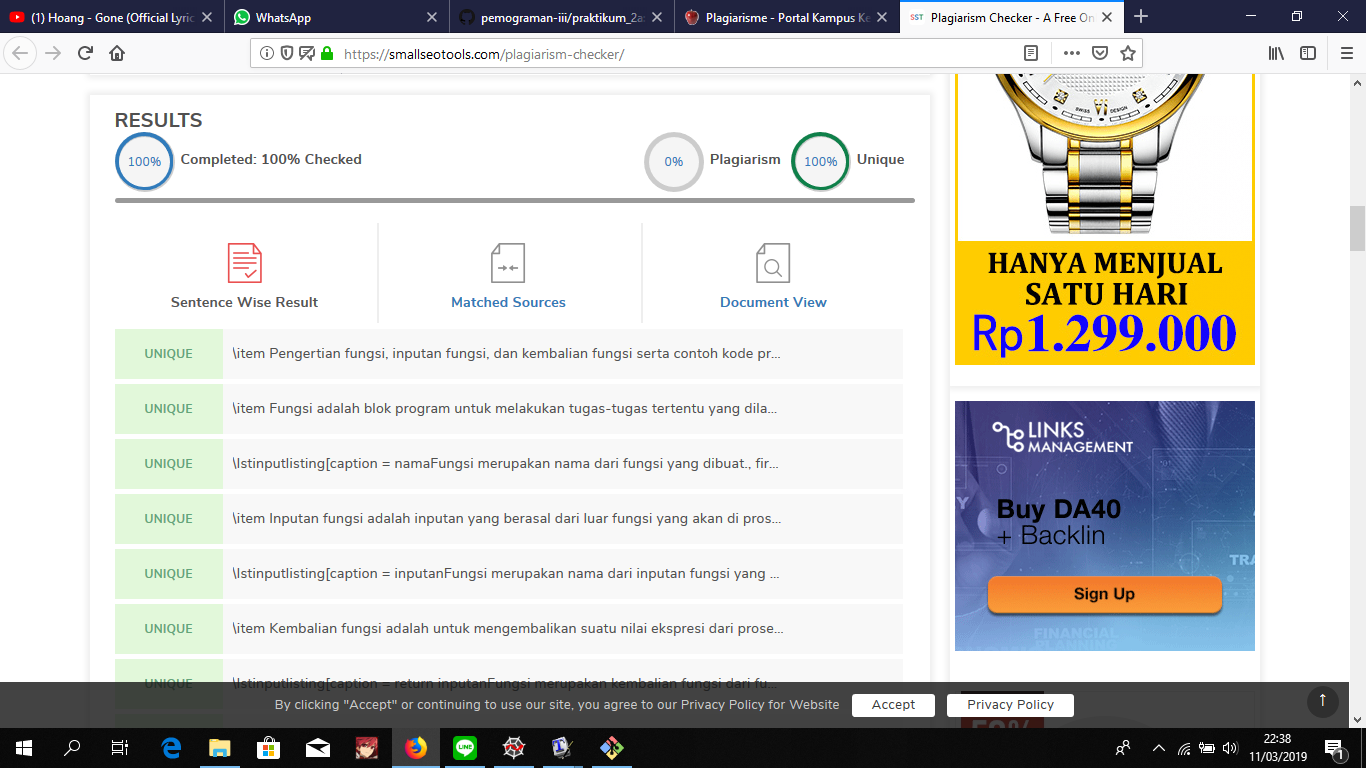
\includegraphics[width=6cm,height=6cm]{figures/habib.png}
\caption{SS Bebas Plagiarisme}
\label{habib}
\end{figure}
%%%%%%%%%%%%%%%%%%%%%%%%%%%%%%%%%%%%%%%%%%%%%%%%%%%%%%
%%%%%%%%%%%%%%%%%%%%%%%%%%%%%%%%%%%%%%%%%%%%%%%%%%%%%%
\section{Dezha Martha}
\subsection{Pemahaman Teori}
\begin{enumerate}
    \item Apa itu fungsi, inputan fungsi dan kembalian fungsi dengan contoh kode program lainnya.
Fungsi memiliki tujuan agar kita dapat memecah program besar menjadi sub-sub program yang lebih sederhana. Pada saat kita membutuhkan suatu fitur maka kita tinggal memanggil fungsi yang telah kita buat. Fungsi pada python dibuat dengan kata kunci def dan diikuti dengan nama fungsi yang kita buat seperti contoh dibawah :
 \lstinputlisting[firstline=10, lastline=10]{src/1174025/1174025.py}
Inputan fungsi merupakan masukan yang kita berikan pada program dan program akan menampilkan hasil dari inputan yang kita masukkan. contoh dari inputan fungsi sebagai berikut :
 \lstinputlisting[firstline=13, lastline=13]{src/1174025/1174025.py}
Pengembalian fungsi memiliki tujuan untuk mengembalikan nilai dari hasil yang telah di proses. Dalam hal ini menggunakan kata kunci return yang diikuti dengan nilai atau variabel yang akan dikembalikan.
 \lstinputlisting[firstline=11, lastline=11]{src/1174025/1174025.py}

    \item Apa itu paket dan cara pemanggilan paket atau library dengan contoh kode program lainnya.
Library atau paket adalah modul-modul yang menyusun python. Modul-modul tersebut ditulis oleh berbagai orang dari seluruh dunia dan memiliki fungsi masing-masing untuk melakukan suatu hal. contoh kode programnya adalah sebagai berikut :
 \lstinputlisting[firstline=16, lastline=18]{src/1174025/1174025.py}

    \item Jelaskan Apa itu kelas, apa itu objek, apa itu atribut, apa itu method dan contoh kode program lainnya masing-masing.
kelas adalah Prototype yang ditentukan oleh pengguna untuk objek yang mendefinisikan seperangkat atribut yang menjadi ciri objek kelas apa pun. Objek ialah instansiasi atau perwujudan dari sebuah kelas. Bila kelas adalah prototipenya, dan objek adalah barang jadinya. Atribut adalah data anggota (variabel kelas dan variabel contoh) dan metode, diakses melalui notasi titik. Sedangkan method fungsi yang didefinisikan di dalam suatu kelas.
 \lstinputlisting[firstline=19, lastline=41]{src/1174025/1174025.py}

    \item Jelaskan cara pemanggilan library kelas dari instansiasi dan pemakaiannya dengan contoh program lainnya.
cara pemanggilan  library kelas dari instansiasi dan pemakaiannya adalah dengan cara meng-import library yang ada di dalam satu folder dan menggunakan kode berikut :
 \lstinputlisting[firstline=42, lastline=52]{src/1174025/1174025.py}

    \item Jelaskan dengan contoh pemakaian paket dengan perintah from kalkulator import Penambahan disertai dengan contoh kode lainnya.
contoh kodenya adalah sebagai berikut :
 \lstinputlisting[firstline=53, lastline=58]{src/1174025/1174025.py}

    \item Jelaskan dengan contoh kodenya, pemakaian paket fungsi apabila file library ada di dalam folder.
 Pemakaian paket adalah perkumpulan fungsi-fungsi. contoh kodenya adalah sebagai berikut :
 \lstinputlisting[firstline=59, lastline=73]{src/1174025/1174025.py}

    \item Jelaskan dengan contoh kodenya, pemakaian paket kelas apabila file library ada di dalam folder.
 \lstinputlisting[firstline=75, lastline=84]{src/1174025/1174025.py}

\end{enumerate}

\subsection{Praktek}
\begin{enumerate}
    \item jawaban no 1
 \lstinputlisting[caption = Jawaban soal no 1.,firstline=90, lastline=126]{src/1174025/1174025.py}

    \item jawaban no 2
 \lstinputlisting[caption = Jawaban soal no 2.,firstline=128, lastline=133]{src/1174025/1174025.py}

    \item jawaban no 3
 \lstinputlisting[caption = Jawaban soal no 3.,firstline=136, lastline=144]{src/1174025/1174025.py}

    \item jawaban no 4
 \lstinputlisting[caption = Jawaban soal no 4.,firstline=145, lastline=150]{src/1174025/1174025.py}

    \item jawaban no 5
 \lstinputlisting[caption = Jawaban soal no 5.,firstline=152, lastline=157]{src/1174025/1174025.py}

    \item jawaban no 6
 \lstinputlisting[caption = Jawaban soal no 6.,firstline=159, lastline=165]{src/1174025/1174025.py}

    \item jawaban no 7
 \lstinputlisting[caption = Jawaban soal no 7.,firstline=167, lastline=173]{src/1174025/1174025.py}

    \item jawaban no 8
 \lstinputlisting[caption = Jawaban soal no 8.,firstline=175, lastline=180]{src/1174025/1174025.py}

    \item jawaban no 9
 \lstinputlisting[caption = Jawaban soal no 9.,firstline=184, lastline=190]{src/1174025/1174025.py}

    \item jawaban no 10
 \lstinputlisting[caption = Jawaban soal no 10.,firstline=192, lastline=208]{src/1174025/1174025.py}

    \item jawaban 11
 \lstinputlisting[caption = Jawaban soal no 11.,firstline=8, lastline=21]{src/1174025/main.py}
 
    \item jawaban 12
 \lstinputlisting[caption = Jawaban soal no 12.,firstline=24, lastline=40]{src/1174025/main.py}
\end{enumerate}

\subsection{Praktek}
\begin{enumerate}
    \item Peringatan error yang ada dan penjelasannya.
    
    \begin{itemize}
    	\item Syntax errors
    	syntax error adalah suatu keadaan saat kode yang dijalankan pada Python menagalami kesalahan penulisan, penempatan dll.
    	Solusi nya adalah dengan menemukan letak sumber masalah dan memperbaikinya.
    	
    	\item Zero Division Error
    	ZeroDivisionError adalah exceptions yang terjadi eksekusi program menghasilkan perhitungan matematika pembagian dengan angka nol (0). Solusiya adalah tidak membagi suatu yang hasilnya nol.
    	\item Name Error
    	NameError adalah exception yang terjadi saat kode melakukan eksekusi terhadap local name atau global name yang tidak terdefinisi. Solusi nya ialah memastikan variabel atau function yang dipanggil ada atau tidak salah ketik.
    	\item Type Error
    	TypeError adalah exception yang terjadi saat dilakukan eksekusi terhadapt suatu operasi atau fungsi dengan tipe objek yang tidak sesuai. Solusinya adalah mengkonversi variabelnya sesuai dengan tipe data yang akan digunakan.
    \end{itemize}
    
    Contoh fungsi yang menggunakan try except
 \lstinputlisting[caption = Penggunaan Try Except .,firstline=214, lastline=221]{src/1174025/1174025.py}

\end{enumerate} 
%%%%%%%%%%%%%%%%%%%%%%%%%%%%%%%%%%%%%%%%%%%%
\section{Damara Benedikta}
\subsection{Pemahaman Teori}
\begin{enumerate}
    \item Apa itu fungsi, inputan fungsi dan kembalian fungsi dengan contoh kode program lainnya.
Fungsi memiliki tujuan agar kita dapat memecah program besar menjadi sub-sub program yang lebih sederhana.pada masing-masing  fitur pada program dapat dibuat dalam satu fungsi. Pada saat kita membutuhkan suatu fitur maka kita tinggal memanggil fungsi yang telah kita buat. Fungsi pada python dibuat dengan menggunakan kata kunci def dan diikuti dengan nama fungsi yang telah kita buat seperti contoh dibawah ini :
 \lstinputlisting[firstline=10, lastline=10]{src/1174012/1174012.py}
Inputan fungsi merupakan masukan yang kita berikan pada program dan program akan menampilkan hasil dari inputan yang telah kita masukkan atau akan menampilkan hasil pada proses selanjutnya. contoh dari inputan fungsi sebagai berikut :
 \lstinputlisting[firstline=11, lastline=11]{src/1174012/1174012.py}
Pengembalian fungsi memiliki tujuan untuk mengembalikan nilai dari hasil yang telah di proses. Dalam hal ini menggunakan kata kunci return yang diikuti dengan nilai atau variabel yang akan dikembalikan.
 \lstinputlisting[firstline=10, lastline=14]{src/1174012/1174012.py}

    \item Apa itu paket dan cara pemanggilan paket atau library dengan contoh kode program lainnya.
Library atau paket adalah modul-modul yang menyusun python. Modul-modul tersebut ditulis oleh berbagai orang dari seluruh dunia dan memiliki fungsi masing-masing untuk melakukan suatu hal. contoh kode programnya adalah sebagai berikut :
 \lstinputlisting[firstline=17, lastline=18]{src/1174012/1174012.py}

    \item Jelaskan Apa itu kelas, apa itu objek, apa itu atribut, apa itu method dan contoh kode program lainnya masing-masing.
kelas adalah Prototype atau blueprint untuk menciptakan suatu object  yang mendefinisikan seperangkat atribut yang menjadi ciri objek kelas apa pun. Objek ialah instansiasi atau perwujudan dari sebuah kelas. Bila kelas adalah prototipenya, dan objek adalah hasil dari class jadinya. Atribut merupakan data dari anggota (variabel kelas, variabel contoh) dan metode, yang diakses dengan notasi titik. Sedangkan method fungsi yang didefinisikan di dalam suatu kelas.
 \lstinputlisting[firstline=21, lastline=40]{src/1174012/1174012.py}

    \item Jelaskan cara pemanggilan library kelas dari instansiasi dan pemakaiannya dengan contoh program lainnya.
cara pemanggilan  library kelas dari instansiasi dan pemakaiannya adalah dengan cara meng-import library yang ada di dalam satu folder dengan menggunakan kode berikut :
 \lstinputlisting[firstline=43, lastline=51]{src/1174012/1174012.py}

    \item Jelaskan dengan contoh pemakaian paket dengan perintah from kalkulator import Penambahan disertai dengan contoh kode lainnya.
contoh kodenya adalah sebagai berikut :
 \lstinputlisting[firstline=54, lastline=57]{src/1174012/1174012.py}

    \item Jelaskan dengan contoh kodenya, pemakaian paket fungsi apabila file library ada di dalam folder.
 Pemakaian paket adalah perkumpulan fungsi-fungsi. contoh kodenya adalah sebagai berikut :
 \lstinputlisting[firstline=60, lastline=73]{src/1174012/1174012.py}

    \item Jelaskan dengan contoh kodenya, pemakaian paket kelas apabila file library ada di dalam folder.
 \lstinputlisting[firstline=76, lastline=84]{src/1174012/1174012.py}

\end{enumerate}

\subsection{Praktek}
\begin{enumerate}
    \item jawaban no 1
 \lstinputlisting[firstline=87, lastline=121]{src/1174012/1174012.py}

    \item jawaban no 2
 \lstinputlisting[firstline=124, lastline=129]{src/1174012/1174012.py}

    \item jawaban no 3
 \lstinputlisting[firstline=132, lastline=139]{src/1174012/1174012.py}

    \item jawaban no 4
 \lstinputlisting[firstline=142, lastline=146]{src/1174012/1174012.py}

    \item jawaban no 5
 \lstinputlisting[firstline=149, lastline=153]{src/1174012/1174012.py}

    \item jawaban no 6
 \lstinputlisting[firstline=156, lastline=161]{src/1174012/1174012.py}

    \item jawaban no 7
 \lstinputlisting[firstline=164, lastline=169]{src/1174012/1174012.py}

    \item jawaban no 8
 \lstinputlisting[firstline=172, lastline=178]{src/1174012/1174012.py}

    \item jawaban no 9
 \lstinputlisting[firstline=181, lastline=186]{src/1174012/1174012.py}

    \item jawaban no 10
 \lstinputlisting[firstline=189, lastline=204]{src/1174012/1174012.py}

    \item jawaban 11
 \lstinputlisting[firstline=8, lastline=22]{src/1174012/main.py}
 \item jawaban 12
 \lstinputlisting[firstline=24, lastline=39]{src/1174012/main.py}
\end{enumerate}

\subsection{Ketrampilan Penanganan Error}
\begin{enumerate}
	\item Peringatan error yang ditemukan dan penjelasannya serta buat sebuah fungsi try except untuk menanggulangi error.
	
	Peringatan error di praktek ketiga ini, yaitu:
	\begin{itemize}
		\item Syntax Errors
		Syntax Errors adalah suatu keadaan saat kode python mengalami kesalahan penulisan. Solusinya adalah memperbaiki penulisan kode yang salah.
		
		\item Zero Division Error
		ZeroDivisonError adalah exceptions yang terjadi saat eksekusi program menghasilkan perhitungan matematika pembagian dengan angka nol (0). Solusinya adalah tidak membagi suatu yang hasilnya nol.
		
		\item Name Error
		NameError adalah exception yang terjadi saat kode melakukan eksekusi terhadap local name atau global name yang tidak terdefinisi. Solusinya adalah memastikan variabel atau function yang dipanggil ada atau tidak salah ketik.
		
		\item Type Error
		TypeError merupakan suatu exception yang terjadi saat akan mengeksekusi suatu operasi atau fungsi dengan type object yang tidak sesuai. Solusinya adalah mengkoversi varibelnya sesuai dengan tipe data yang akan digunakan.
	\end{itemize}
   \end{enumerate}

   \begin{figure}
   \centering
   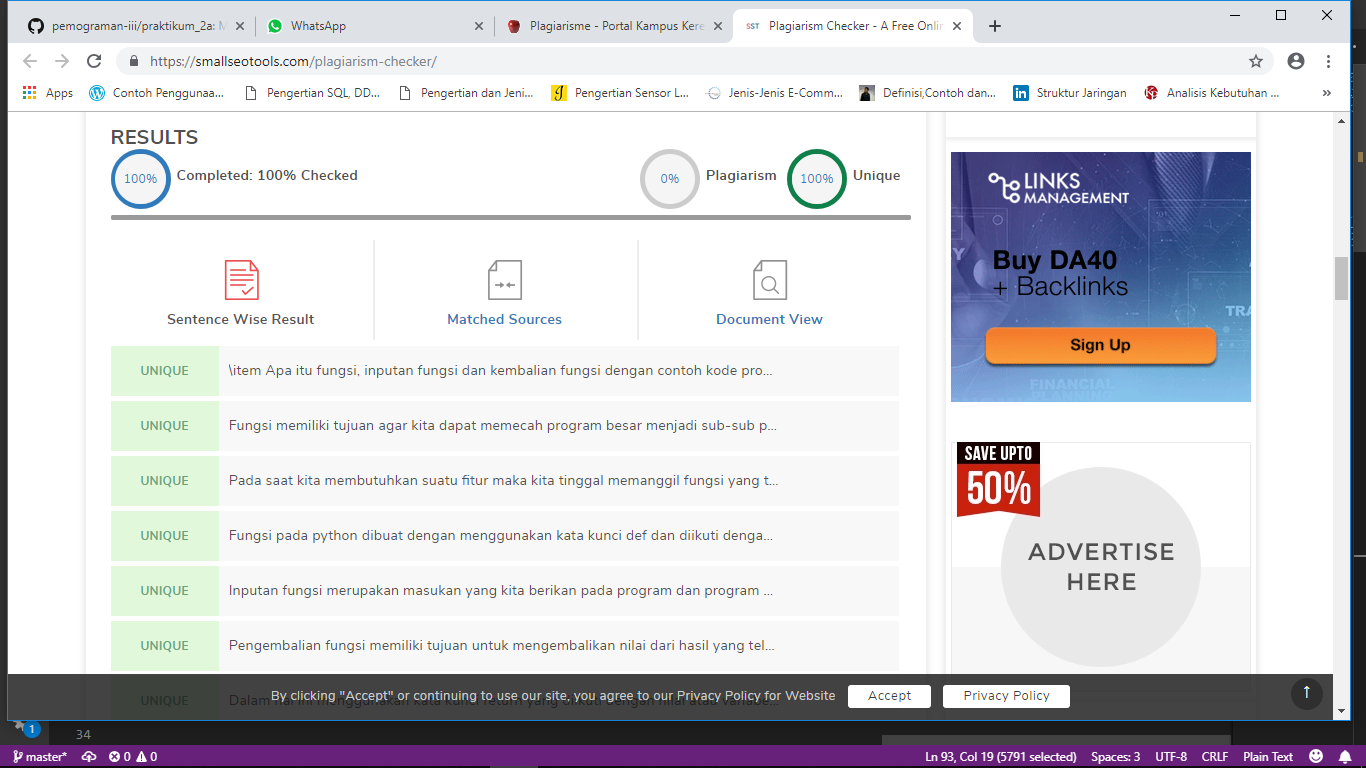
\includegraphics[width=6cm,height=6cm]{figures/damaraa.png}
   \caption{SS plagiarisme}
   \label{damara}
   \end{figure}

%%%%%%%%%%%%%%%%%%%%%%%%%%%%%%%%%%%%%%%%%%%%%%%%%%%%%%%%%%%%%%%%%%%%%%%%%%%

%%%%%%%%%%%%%%%%%%%%%%%%%%%%%%%%%%%%%%%%%%%%%%%%%%%%%%%%%%%%%%
\section{Arjun Yuda Firwanda}
\subsubsection{Pemahanan Teori}
\begin{enumerate}
    \item Apa itu fungsi, inputan fungsi dan kembalian fungsi dengan contoh kode program
    lainnya.
    Fungsi merupakan pendefinisian dengan kata kunci def dan diikuti parameter.
    \lstinputlisting[firstline=126, lastline=129]{src/1174008.py}

    Fungsi juga dapat membaca parameter, parameter adalah nilai yang disediakan kepada fungsi yang akan menentukan output yang akan dihasilkan fungsi.
    \lstinputlisting[firstline=131, lastline=134]{src/1174008.py}

    Perintah return digunakan untuk keluar dari fungsi. Kita juga dapat menspesifikasikan nilai kembalian.
    \lstinputlisting[firstline=136, lastline=143]{src/1174008.py}

    \item Apa itu paket dan cara pemanggilan paket atau library dengan contoh kode
    program lainnya.
    Paket untuk memudahkan dalam pemanggilan fungsi yang di butuhkan agar dapat dipanggil secara berulang.
    Cara pemanggilannya
    \lstinputlisting[firstline=145, lastline=146]{src/1174008.py}

    \item Jelaskan Apa itu kelas, apa itu objek, apa itu atribut, apa itu method dan
    contoh kode program lainnya masing-masing.
    Kelas merupakan blueprint cetakan atau kerangka dasar dari objek.
    Objek merupakan instance yang mempresentasikan nyata dari sebuah class.
    Method merupakan suatu operasi yang berupa fungsi-fungsi yang dikerjakan oleh sebuah objek.
    Attribute merupakan instan spesifik dari setiap objek.
    \lstinputlisting[firstline=148, lastline=170]{src/1174008.py}

    \item Jelaskan cara pemanggikan library kelas dari instansiasi dan pemakaiannya den-
    gan contoh program lainnya.
    Cara Pemanggilanya 
    \begin{itemize}
        \item pertama import terlebih dahulu filenya.
        \item kemudian buat variabel untuk menampung datanya.
        \item setelah itu panggil nama classnya dan panggil methodnya.
        \item Gunakan perintah print untuk menampilkan hasilnya.

    \end{itemize}
    \lstinputlisting[firstline=172, lastline=177]{src/1174008.py}

    \item Jelaskan dengan contoh pemakaian paket dengan perintah from kalkulator im-
    port Penambahan disertai dengan contoh kode lainnya.
    Penggunaan paket from namafile import yaitu berfungsi memanggil file dan fungsinya.
    \lstinputlisting[firstline=145, lastline=146]{src/1174008.py}

    \item Jelaskan dengan contoh kodenya, pemakaian paket fungsi apabila le library
    ada di dalam folder.
    Pemakaian paket merupakan sekumpulan fungsi-fungsi. contoh kodenya adalah sebagai berikut:

    \item Jelaskan dengan contoh kodenya, pemakaian paket kelas apabila le library ada
    di dalam folder.
    \lstinputlisting[firstline=186, lastline=186]{src/1174008.py}

\end{enumerate}
\subsubsection{Ketrampilan Pemrograman}
\begin{enumerate}
    \item Buatlah fungsi dengan inputan variabel NPM, dan melakukan print luaran huruf
    yang dirangkai dari tanda bintang, pagar atau plus dari NPM kita. Tanda
    bintang untuk NPM mod 3=0, tanda pagar untuk NPM mod 3 =1, tanda plus
    untuk NPM mod3=2.
    \lstinputlisting[firstline=186, lastline=236]{src/1174008.py}

    \item Buatlah fungsi dengan inputan variabel berupa NPM. kemudian dengan meng-
    gunakan perulangan mengeluarkan print output sebanyak dua dijit belakang
    NPM.
    \lstinputlisting[firstline=240, lastline=244]{src/1174008.py}

    \item Buatlah fungsi dengan dengan input variabel string bernama NPM dan beri
    luaran output dengan perulangan berupa tiga karakter belakang dari NPM se-
    banyak penjumlahan tiga dijit tersebut.
    \lstinputlisting[firstline=247, lastline=254]{src/1174008.py}

    \item Buatlah fungsi hello word dengan input variabel string bernama NPM dan
    beri luaran output berupa digit ketiga dari belakang dari variabel NPM meng-
    gunakan akses langsung manipulasi string pada baris ketiga dari variabel NPM.
    \lstinputlisting[firstline=257, lastline=260]{src/1174008.py}

    \item buat fungsi program dengan input variabel NPM dan melakukan print nomor npm satu persatu kebawah.
    \lstinputlisting[firstline=263, lastline=265]{src/1174008.py}

    \item Buatlah fungsi dengan inputan variabel NPM, didalamnya melakukan penjum-
    lahan dari seluruh dijit NPM tersebut, wajib menggunakan perulangan dan
    atau kondisi.
    \lstinputlisting[firstline=267, lastline=272]{src/1174008.py}

    \item Buatlah fungsi dengan inputan variabel NPM, didalamnya melakukan melakukan
    perkalian dari seluruh dijit NPM tersebut, wajib menggunakan perulangan dan
    atau kondisi.
    \lstinputlisting[firstline=274, lastline=279]{src/1174008.py}

    \item Buatlah fungsi dengan inputan variabel NPM, Lakukan print NPM anda tapi
    hanya dijit genap saja. wajib menggunakan perulangan dan atau kondisi.
    \lstinputlisting[firstline=281, lastline=286]{src/1174008.py}

    \item Buatlah fungsi dengan inputan variabel NPM, Lakukan print NPM anda tapi
    hanya dijit ganjil saja. wajib menggunakan perulangan dan atau kondisi.
    \lstinputlisting[firstline=288, lastline=293]{src/1174008.py}

    \item Buatlah fungsi dengan inputan variabel NPM, Lakukan print NPM anda tapi
    hanya dijit yang termasuk bilangan prima saja. wajib menggunakan perulangan
    dan atau kondisi.
    \lstinputlisting[firstline=295, lastline=308]{src/1174008.py}

    \item Buatlah satu library yang berisi fungsi-fungsi dari nomor diatas dengan nama
    le 3lib.py dan berikan contoh cara pemanggilannya pada le main.py.
    \lstinputlisting[firstline=7, lastline=7]{src/main.py}

    \item Buatlah satu library class dengan nama le kelas3lib.py yang merupakan mod-
    ikasi dari fungsi-fungsi nomor diatas dan berikan contoh cara pemanggilannya
    pada le main.py.
    \lstinputlisting[firstline=8, lastline=9]{src/main.py}
    
\end{enumerate}
\subsubsection{Ketrampilan Penanganan Error}
Error yang di dapat dari mengerjakan tugas ini adalah type error, cara menaggulaginya dengan cara mengecheck kembali codingannya
kemudian run kembali aplikasinya
berikut contoh Penggunaan fungsi try dan exception
\lstinputlisting[firstline=177, lastline=182]{src/1174008.py}



\section{Muhammad Fahmi}
\textbf{{\large Fungsi dan Kelas}}

\subsection{Pemahaman Teori}
\begin{enumerate}
	\item Fungsi adalah bagian dari program yang dapat digunakan ulang, kemudian nama ini dapat dipanggil di manapun dalam program.
	Contoh fungsi dan pemanggilannya adalah :
	\lstinputlisting[caption=Penggunaan fungsi, frame=single, firstline=3, lastline=6]{src/1174021/1174021.py}
	Fungsi juga dapat membaca parameter, parameter tersebut berupa nilai yang disediakan kepada fungsi, dimana nilai ini akan menentukan output yang akan dihasilkan fungsi. 
	\lstinputlisting[caption=Penggunaan fungsi,frame=single, firstline=8, lastline=12]{src/1174021/1174021.py}
	Didalam fungsi juga ada Statemen return yang digunakan untuk keluar dari fungsi. Kita juga dapat menspesifikasikan nilai kembalian.
	\lstinputlisting[caption=Penggunaan return,frame=single, firstline=14, lastline=21]{src/1174021/1174021.py}
	
	\item Paket didalam Python juga dikatakan Modul,  adalah sebuah file yang berisi kode python, misalnya: coba.py 
	Cara pemanggilan paket atau library yaitu dengan meng-import paket atau library yang akan digunakan. Kemudian panggil dengan cara mendefinisikan.
	\lstinputlisting[caption=Penggunaan paket atau library, frame=single, firstline=24, lastline=25]{src/1174021/1174021.py}
	
	\item \begin{itemize}
		\item Kelas
		Kelas adalah berupa blueprint atau cetak biru dari sebuah objek dimana kita mendefinisikan atribut dari suatu objek tersebut.
		Contoh penggunaan kelas adalah : 
		\lstinputlisting[caption = Penggunaan kelas di python, firstline=28, lastline=47]{src/1174021/1174021.py}
		
		\item Objek
		Objjek adalah sebuah contoh unik dari struktur data yang didefinisikan oleh kelasnya. Objek juga terdiri dari beberapa anggota data dan metode.
		\lstinputlisting[caption = Penggunaan objek di python, firstline=39, lastline=42]{src/1174021/1174021.py}
		
		\item Atribut
		Atribut adalah variabel yang menyimpan data yang berhubungan dengan kelas dan objeknya.
		\lstinputlisting[caption = Penggunaan atribut di python, firstline=29, lastline=29]{src/1174021/1174021.py}
		
		\item Method
		Methode atau moetode adalah sebuah jenis fungsi khusus yang didefinisikan dalam definisi kelas.
		\lstinputlisting[caption = Penggunaan method di python, firstline=35, lastline=37]{src/1174021/1174021.py}
		
	\end{itemize}
	
	
	\item Cara pemanggikan library kelas dari instansiasi dan pemakaiannya, berikut adalah contohnya : 
	\lstinputlisting[caption = Pemanggilan libraby kelas, firstline=50, lastline=60]{src/1174021/1174021.py}
	
	\item Pemakaian paket dengan perintah from kalkulator import Penambahan, berikut adalah contohnya : 
	\lstinputlisting[caption = Pemakaian paket from kalkulator import penambahan, firstline=63, lastline=66]{src/1174021/1174021.py}
	
	\item Pemakaian paket fungsi apabila file library ada di dalam folder, berikut adalah contohnya : 
	\lstinputlisting[caption = Pemakaian paket fungsi, firstline=69, lastline=82]{src/1174021/1174021.py}
	
	\item Pemakaian paket kelas apabila file library ada di dalam folder, berikut adalah contohnya : 
	\lstinputlisting[caption = Pemakaian paket fungsi2, firstline=85, lastline=95]{src/1174021/1174021.py}
	
\end{enumerate}

Hasil tampilan pemahaman teori : 
\begin{figure}[h]
	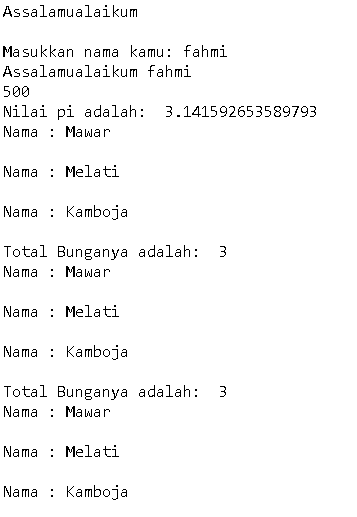
\includegraphics[width=50mm]{figures/fahmi/5.png}
	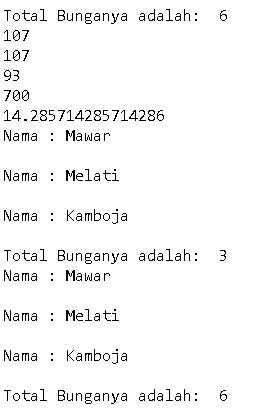
\includegraphics[width=50mm]{figures/fahmi/6.png}
	\centering
\end{figure}


\newpage
\subsection{Keterampilan Program}
\begin{enumerate}
	\item Jawaban Soal 1
	\lstinputlisting[caption = Jawaban Soal 1, firstline=101, lastline=146]{src/1174021/1174021.py}
	
	\item Jawaban Soal 2
	\lstinputlisting[caption = Jawaban Soal 2, firstline=149, lastline=157]{src/1174021/1174021.py}
	
	\item Jawaban Soal 3
	\lstinputlisting[caption = Jawaban Soal 3, firstline=160, lastline=168]{src/1174021/1174021.py}
	
	\item Jawaban Soal 4
	\lstinputlisting[caption = Jawaban Soal 4, firstline=171, lastline=177]{src/1174021/1174021.py}
	
	\item Jawaban Soal 5
	\lstinputlisting[caption = Jawaban Soal 5, firstline=180, lastline=187]{src/1174021/1174021.py}
	
	\item Jawaban Soal 6
	\lstinputlisting[caption = Jawaban Soal 6, firstline=190, lastline=197]{src/1174021/1174021.py}
		
	\item Jawaban Soal 7
	\lstinputlisting[caption = Jawaban Soal 7, firstline=200, lastline=207]{src/1174021/1174021.py}
	
	\item Jawaban Soal 8
	\lstinputlisting[caption = Jawaban Soal 8, firstline=210, lastline=217]{src/1174021/1174021.py}
	
	\item Jawaban Soal 9
	\lstinputlisting[caption = Jawaban Soal 9, firstline=220, lastline=228]{src/1174021/1174021.py}
	
	\item Jawaban Soal 10
	\lstinputlisting[caption = Jawaban Soal 9, firstline=231, lastline=248]{src/1174021/1174021.py}
	
	\item Jawaban Soal 11
	\lstinputlisting[caption = Jawaban Soal 9, firstline=1, lastline=3]{src/1174021/main.py}
	
	\item Jawaban Soal 12
	\lstinputlisting[caption = Jawaban Soal 9, firstline=7, lastline=11]{src/1174021/main.py}
	
\end{enumerate}

\subsection{Keterampilan Penanganan Error}
\begin{enumerate}
	\item Peringatan error yang ditemukan dan penjelasannya serta buat sebuah fungsi try except untuk menanggulangi error.
	
	Jenis-jenis error pada praktek kali ini adalah :
	\begin{itemize}
	\item Syntax Errors
	Syntax Errors adalah suatu keadaan dimana kode python mengalami kesalahan penulisan. Solusinya adalah memperbaiki penulisan kode yang salah.
	
	\item Zero Division Error
	ZeroDivisonError adalah sebuah exceptions yang terjadi saat kita mengeksekusi sebuah program kemudian menghasilkan perhitungan matematika pembagian dengan angka nol (0) solusinya adalah tidak membagi suatu yang hasilnya nol.
	
	\item Name Error
	NameError adalah sebuah exceptions yang terjadi jika sebuah kode melakukan eksekusi terhadap local name atau global name yang tidak terdefinisi. Solusinya adalah dengan memastikan variabel atau function yang telah dipanggil ada atau tidak salah ketik.
	
	\item Type Error
	TypeError adalah sebuah exceptions yang terjadi pada saat melakukan eksekusi terhadap suatu operasi atau fungsi dengan type object yang tidak sesuai. Solusinya adalah dengan mengkoversi varibelnya sesuai dengan tipe data yang akan digunakan.
	\end{itemize}
	
	Contoh fungsi yang menggunakan try except
	\lstinputlisting[caption= Fungsi yang menggunakan try except ,firstline=255, lastline=261]{src/1174021/1174021.py}
\end{enumerate}


\section{Muhammad Dzihan Al-Banna}
\subsection{Pemahaman Teori}
\subsubsection{Apa itu fungsi}
Fungsi adalah sebuah program yang dapat digunakan ulang. Sebuah fungsi dapat digunakan ulang dengan cara memberi nama pada blok statemen kemudian nama tersebut dapat dipanggil dalam program lain. 
\lstinputlisting[caption = contoh fungsi, firstline=8, lastline=11]{src/1174095/persib.py}
Inputan fungsi adalah sebuah fungsi yang mempunyai interkasi dengan user dan dapat menginputkan value.
\lstinputlisting[caption = contoh input fungsi, firstline=14, lastline=17]{src/1174095/persib.py}
Kembalian fungsi adalah hasil yang dikembalikan dari inputan.
\lstinputlisting[caption = contoh fungsi yang menghasilkan kembalian, firstline=20, lastline=127]{src/1174095/persib.py} 
\subsubsection{Apa itu paket}
Package adalah suatu teknik pengemasan modul di dalam python. Package menyediakan kemampuan bagi programmer untuk mengelompokkan modul yang telah dibuat. untuk pemanggilan sebuah package maka perlu dibuat dulu package yang akan dipanggil dan cara memanggilnya seperti berikut :
\lstinputlisting[caption = pakcage, firstline=28, lastline=31]{src/1174095/persib.py}

\subsubsection{Apa itu kelas, objek dan atribut}
kelas adalah Prototipe yang ditentukan oleh pengguna untuk sebuah objek yang mendefinisikan seperangkat atribut yang menjadi ciri objek kelas.
\lstinputlisting[caption = kelas python, firstline=32, lastline=49]{src/1174095/persib.py}
Atribut adalah data anggota dan metode,dapat diakses melalui notasi titik.
Objek adalah Contoh unik dari struktur yang didefinisikan oleh kelas. 
Objek terdiri dari kedua anggota data (variabel kelas dan variabel contoh) dan metode.
\lstinputlisting[caption = objek, firstline=43, lastline=44]{src/1174095/persib.py}
dan atribut seperti code di bawah ini :
\lstinputlisting[caption = atribut, firstline=49, lastline=49]{src/1174095/persib.py}
\subsubsection{pemanggilan library}
Dalam pemanggilan sebuah package ada langkah-langkah yang harus dikerjakan seperti langkah berikut ini :
\begin{enumerate}
	\item Import dahulu paket yang akan dipanggil
	\item buat variabel
	\item panggil method dan class
	\item buat print untuk menampilkan hasilnya
	print("Sepedanya ", Sepeda.jumlahSepeda)
	\lstinputlisting[caption = pemanggilan pakcage, firstline=52, lastline=60]{src/1174095/persib.py}
\end{enumerate}
\subsubsection{Pemakaian paket}
\lstinputlisting[caption = pemakaian package, firstline=62, lastline=62]{src/1174095/persib.py}
\subsubsection{Paket fungsi file di dalam folder}
\lstinputlisting[caption = pemanggilan file dalam folder, firstline=64, lastline=68]{src/1174095/persib.py}
\subsubsection{Paket kelas file di dalam folder}
\lstinputlisting[caption = pemakaian package kelas di luar folder, firstline=62, lastline=62]{src/1174095/persib.py}
\subsection{Keterampilan Pemrograman}
\begin{enumerate}
	\item Tugas 1
	\lstinputlisting[caption = tugas 1, firstline=9, lastline=43]{src/1174095/radovic.py}
	\begin{figure}
		
		\caption{}
	\end{figure}
	\item Tugas 2
	\lstinputlisting[caption = pemakaian package, firstline=46, lastline=51]{src/1174095/radovic.py}
	\item Tugas 3
	\lstinputlisting[caption = pemakaian package, firstline=54, lastline=61]{src/1174095/radovic.py}
	\item Tugas 4
	\lstinputlisting[caption = pemakaian package, firstline=64, lastline=68]{src/1174095/radovic.py}
	\item Tugas 5
	\lstinputlisting[caption = pemakaian package, firstline=71, lastline=75]{src/1174095/radovic.py}
	\item Tugas 6
	\lstinputlisting[caption = pemakaian package, firstline=78, lastline=83]{src/1174095/radovic.py}
	\item Tugas 7
	\lstinputlisting[caption = pemakaian package, firstline=86, lastline=91]{src/1174095/radovic.py}
	\item Tugas 8
	\lstinputlisting[caption = pemakaian package, firstline=94, lastline=100]{src/1174095/radovic.py}
	\item Tugas 9
	\lstinputlisting[caption = pemakaian package, firstline=103, lastline=108]{src/1174095/radovic.py}
	\item Tugas 10
	\lstinputlisting[caption = pemakaian package, firstline=112, lastline=127]{src/1174095/radovic.py}
	\item Tugas 11
	\lstinputlisting[caption = pemakaian package, firstline=1, lastline=3]{src/1174095/main.py}
	\item Tugas 12
	\lstinputlisting[caption = pemakaian package, firstline=5, lastline=9]{src/1174095/main.py}
\end{enumerate}
\subsection{Keterampilan Penanganan Error}
\begin{enumerate}
	\item Peringatan error yang ditemukan dan penjelasannya serta buat sebuah fungsi try except untuk menanggulangi error.
	
	Peringatan error di praktek ketiga ini, yaitu:
	\begin{itemize}
		\item Syntax Errors
		Syntax Errors adalah suatu keadaan disaat kode mengalami kesalahan penulisan. Cara menanganinya adalah dengan memperbaiki penulisan kode yang salah.
		
		\item Zero Division Error
		Zero Divison Error adalah exceptions yang terjadi saat eksekusi program menghasilkan perhitungan matematika pembagian dengan angka nol (0). Solusinya adalah tidak membagi suatu yang hasilnya nol.
		
		\item Name Error
		NameError adalah exception yang terjadi saat melakukan eksekusi terhadap local name atau global name yang tidak terdefinisi. Solusinya adalah memastikan bahwa variabel atau function yang dipanggil tidak salah penulisan.
		
		\item Type Error
		TypeError adalah exception yang terjadi saat melakukan eksekusi terhadap suatu operasi atau fungsi dengan type object yang tidak sesuai. Solusinya adalah mengkoversi varibelnya sesuai dengan tipe data yang akan digunakan.
		\lstinputlisting[caption = pemakaian package, firstline=131, lastline=137]{src/1174095/radovic.py}
	\end{itemize}
\end{enumerate}

\section{Hasil}
\begin{itemize}
	\item Hasil
	\begin{figure}[H]
		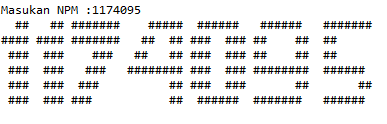
\includegraphics[width=10cm]{figures/dzihan/hasil.png}
		\centering
	\end{figure}
	\item Hasil 2
	\begin{figure}[H]
		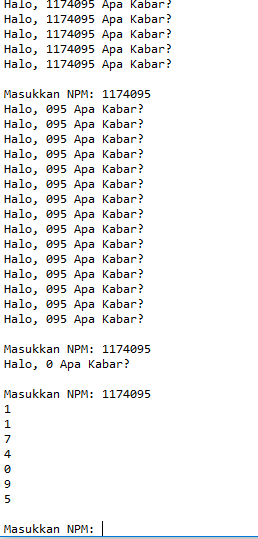
\includegraphics[width=10cm]{figures/dzihan/2f.png}
		\centering
	\end{figure}
	\item hasil 3
	\begin{figure}[H]
		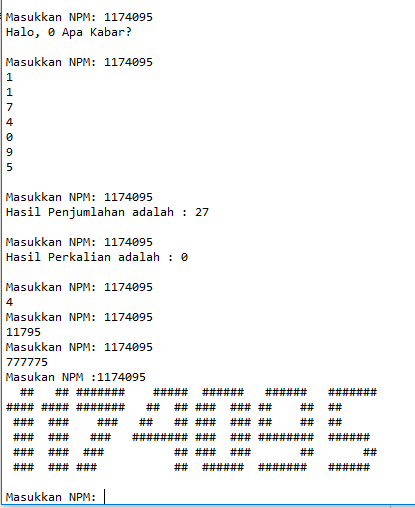
\includegraphics[width=10cm]{figures/dzihan/3.png}
		\centering
	\end{figure}
\end{itemize}

%%%%%%%%%%%%%%%%%%%%%%%%%
\section{Nico Ekklesia Sembiring}
\subsection{Tugas Teori}
\begin{enumerate}
	\item Apa itu fungsi, inputan fingsi dan kembalian fungsi dengan contoh kode program
	lainnya.\newline
	Fungsi merupakan suatu blok program yang terdiri atas nama fungsi, input variabel, dan kembalian variabel. 
	Fungsi pada python dibuat dengan kata kunci "def" dan diikuti dengan nama fungsi. contohnya adalah:
	\lstinputlisting[firstline=10, lastline=14]{src/1174096/1174096.py}
	
	\item Apa itu paket dan cara pemanggilan paket atau library dengan contoh kode program lainnya.\newline
	Library atau paket adalah modul-modul yang menyusun python. Modul-modul tersebut ditulis oleh berbagai orang dari seluruh dunia dan memiliki fungsi masing-masing untuk melakukan suatu hal. contoh kode programnya adalah sebagai berikut :
	\lstinputlisting[firstline=17, lastline=18]{src/1174096/1174096.py}
	
	\item Jelaskan Apa itu kelas, apa itu objek, apa itu atribut, apa itu method dan contoh kode program lainnya masing-masing.\newline
	Kelas adalah Prototype yang ditentukan oleh pengguna untuk objek yang mendefinisikan seperangkat atribut yang menjadi ciri objek kelas apa pun. Objek ialah instansiasi atau perwujudan dari sebuah kelas. Contoh dapat dilihat sebagai berikut :
	\lstinputlisting[firstline=21, lastline=39]{src/1174096/1174096.py}
	
	\item Jelaskan cara pemanggikan library kelas dari instansiasi dan pemakaiannya dengan contoh program lainnya.\newline
	Cara pemanggilan  library kelas dari instansiasi dan pemakaiannya adalah dengan cara meng-import library yang ada di dalam satu folder dan menggunakan kode berikut :
	\lstinputlisting[firstline=42, lastline=50]{src/1174096/1174096.py}
	
	\item Jelaskan dengan contoh pemakaian paket dengan perintah from kalkulator import Penambahan disertai dengan contoh kode lainnya.\newline
	Penggunaan paket dengan perintah from kalkulator berfungsi untuk memanggil file dan fungsinya. contoh kodenya adalah sebagai berikut :
	\lstinputlisting[firstline=53, lastline=56]{src/1174096/1174096.py}
	
	\item Jelaskan dengan contoh kodenya, pemakaian paket fungsi apabila file library ada di dalam folder.\newline
	Pemakaian paket adalah perkumpulan fungsi-fungsi. contoh kodenya adalah sebagai berikut :
	\lstinputlisting[firstline=59, lastline=72]{src/1174096/1174096.py}
	
	\item Jelaskan dengan contoh kodenya, pemakaian paket kelas apabila file library ada
	di dalam folder.\newline
	\lstinputlisting[firstline=75, lastline=83]{src/1174096/1174096.py}
\end{enumerate}

\subsection{Tugas Keterampilan Pemrograman}
\begin{enumerate}
	\item Buatlah fungsi dengan inputan variabel NPM, dan melakukan print luaran huruf yang dirangkai dari tanda bintang, pagar atau plus dari NPM kita. Tanda bintang untuk NPM mod 3=0, tanda pagar untuk NPM mod 3 =1, tanda plus untuk NPM mod3=2.
	\lstinputlisting[firstline=89, lastline=123]{src/1174096/1174096.py}
	
	\item Buatlah fungsi dengan inputan variabel berupa NPM. kemudian dengan menggunakan perulangan mengeluarkan print output sebanyak dua dijit belakang
	NPM.
	\lstinputlisting[firstline=126, lastline=131]{src/1174096/1174096.py}
	
	\item Buatlah fungsi dengan dengan input variabel string bernama NPM dan beri
	luaran output dengan perulangan berupa tiga karakter belakang dari NPM sebanyak penjumlahan tiga dijit tersebut. Penjumlahan dilakukan dengan menggunakan operator aritmatika dan fungsi int() atau str().
	\lstinputlisting[firstline=134, lastline=141]{src/1174096/1174096.py}
	
	\item Buatlah fungsi hello word dengan input variabel string bernama NPM dan beri luaran output berupa digit ketiga dari belakang dari variabel NPM menggunakan akses langsung manipulasi string pada baris ketiga dari variabel NPM.
	\lstinputlisting[firstline=144, lastline=148]{src/1174096/1174096.py}
	
	\item Buat fungsi program dengan input variabel NPM dan melakukan print nomor npm satu persatu kebawah.
	\lstinputlisting[firstline=151, lastline=155]{src/1174096/1174096.py}
	
	\item Buatlah fungsi dengan inputan variabel NPM, didalamnya melakukan penjumlahan dari seluruh dijit NPM tersebut, wajib menggunakan perulangan dan
	atau kondisi.
	\lstinputlisting[firstline=158, lastline=163]{src/1174096/1174096.py}
	
	\item Buatlah fungsi dengan inputan variabel NPM, didalamnya melakukan melakukan perkalian dari seluruh dijit NPM tersebut, wajib menggunakan perulangan dan atau kondisi.
	\lstinputlisting[firstline=166, lastline=171]{src/1174096/1174096.py}
	
	\item Buatlah fungsi dengan inputan variabel NPM, Lakukan print NPM anda tapi hanya dijit genap saja. wajib menggunakan perulangan dan atau kondisi
	\lstinputlisting[firstline=174, lastline=180]{src/1174096/1174096.py}
	
	\item Buatlah fungsi dengan inputan variabel NPM, Lakukan print NPM anda tapi hanya dijit ganjil saja. wajib menggunakan perulangan dan atau kondisi..
	\lstinputlisting[firstline=183, lastline=188]{src/1174096/1174096.py}
	
	\item Buatlah fungsi dengan inputan variabel NPM, Lakukan print NPM anda tapi hanya dijit yang termasuk bilangan prima saja. wajib menggunakan perulangan dan atau kondisi..
	\lstinputlisting[firstline=191, lastline=206]{src/1174096/1174096.py}
	
	\item Buatlah satu library yang berisi fungsi-fungsi dari nomor diatas dengan nama file 3lib.py dan berikan contoh cara pemanggilannya pada file main.py.
	\lstinputlisting[firstline=8, lastline=21]{src/1174096/main.py}
	
	\item Buatlah satu library class dengan nama file kelas3lib.py yang merupakan modifikasi dari fungsi-fungsi nomor diatas dan berikan contoh cara pemanggilannya pada file main.py..
	\lstinputlisting[firstline=23, lastline=38]{src/1174096/main.py}
	
\end{enumerate}
\subsection{Ketrampilan Penanganan Error}
\lstinputlisting[firstline=209, lastline=214]{src/1174096/1174096.py}

\subsection{Cek Plagiarisme}
\begin{figure}[!htbp]
	\centering
	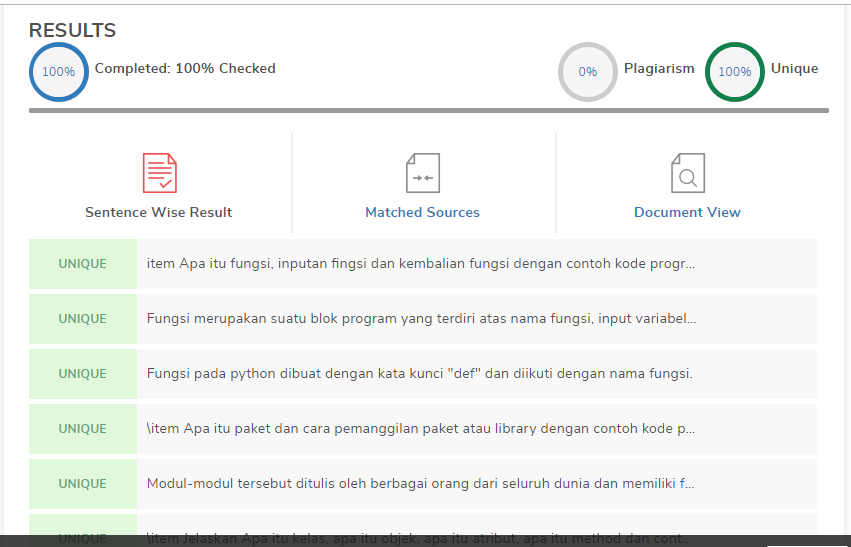
\includegraphics[width=3cm,height=3cm]{figures/nico/plagiarisme.png}
	\caption{Plagiarisme}
	\label{plagiarisme}
\end{figure}